\chapter{Beam Modulation}
%\chapter{BEAM MODULATION}
\label{BEAM MODULATION 2}
%\index{Beam Modulation}

\section{Beam Modulation\index{Beam Modulation}}
\label{Beam Modulation 2}


\begin{equation} \label{equ:time1}
dA = \frac{1}{\sqrt{N}} = 1\times10^{-6} = 1~ppm
\end{equation}

\begin{equation} \label{equ:time2}
N = 10^{12}~\text{counts} = Rt
\end{equation}

\begin{equation} \label{equ:time3}
t = \frac{N}{R} = \frac{10^{12}}{8\times800\times10^{6}~Hz} = 156.25~s
\end{equation}


%\subsection{Introduction}
%\label{Introduction2}
%
%The $Q_{weak}^p$ experiment will measure the parity violating asymmetry ($~$234 ppb) in elastic electron-proton scattering to determine the proton s weak charge with 4~\% total uncertainty. The e+p scattering rate depends in first order on the five beam parameters at the scattering target: horizontal position (X), horizontal angle (X$^{'}$), vertical position (Y), vertical angle (Y$^{'}$), and energy (E). Small changes in these parameters will create a change in rate which, if beam helicity dependent, would create a false asymmetry. While the source group tries to keep these helicity-correlated parameter changes as small as possible, the goal of our beam modulation group is to occasionally induce controlled beam parameter changes $dX_i$, measure the resulting detector false asymmetry $A_i^{false}$, and determine the detector sensitivities $A_i^{false}/dX_i$. This will allow later correction of beam false asymmetries via $A_{correction}$ = i=1,5 $(A_i^{false}/dXi)*Xi$.  Even if these corrections prove to be small under ideal running conditions, the modulation system described here will allow us to quickly determine if undesirable changes have occurred. 
%
%\subsection{Measurement Time vs Modulation Asymmetry}
%\label{Measurement Time vs Modulation Asymmetry}
%We begin with the assumption that it would be helpful to measure the whole-detector sensitivities to 10\% accuracy every few days (provided it can be done using only a small fraction of our beam time and without beam strikes or halo scraping).  If the sensitivities prove to be stable, this would yield few percent errors by the end of the experiment. This is much better than one would need to regress out the helicity-correlated differences seen in the last HAPPEx Hydrogen run. [ref: A. Acha et al., Precision Measurements of the Nucleon Strange Form Factors at Q2 ~0.1 GeV2, PRL 98, 032301 (2007)]   However, frequent whole-detector sensitivity measurements might reveal important changes in beam or target cell position, the presence of an unmeasured beam parameter, or even a broken glue joint in the main detector. Furthermore, accurate single-octant sensitivities (which would be obtained as a by-product) are an essential prerequisite to extracting the $\sin\phi$ and $\cos\phi$ dependences which are symptomatic of residual transverse beam polarization.
%
%For the size and duration of the modulations we discuss below, the natural beam jitter and the SEE BPM electronic noise of roughly 5?m/?Hz will be negligible. (Were this not the case, measurement times would become much longer.) This means the error on the detector sensitivities is dominated by the statistical error on the detector false asymmetry.  At nominal luminosity, the $Q_{weak}^{p}$ experiment has a rate of 800 MHz /octant, hence the whole-detector statistical sensitivity dA = 12.5 ppm/?t(sec), or 1 ppm in 156.25 seconds. The clock times needed to measure a single beam sensitivity to 10\% are therefore
%
%\begin{equation} \label{equ:time}
%t (s) = \frac{1}{DF} \frac{12.5 ppm}{A(ppm)^2}\frac{dA}{A} = 
%\end{equation}
%
%t (sec) = (1/DF)* (12.5 ppm/A(ppm))2/(dA/A)2 = (1/DF)*100*(12.5ppm/A(ppm))2 . 
%
%
%\begin{singlespace}
%\begin{table}[!h]
%\begin{center}
%  	\caption
%	[Dead time calculation for beam modulation.]
%  	{Dead time calculation for beam modulation. The clock time needed to measure detector sensitivity for a single parameter and how it varies with asymmetries are shown here.}
%  \begin{tabular}{ c | c | c | c }
%%    \hline
%    \noalign{\hrule height 1pt}
%    \multirow{2}{*}{Modulation asymmetry} & \multicolumn{3}{c}{Clock time required} \\
%    \cline{2-4}
%     & 10\% DF & 1\% DF & 0.1\% DF \\
%     $\left[ \text{ppm}\right]$ & [Hours] & [Hours] & [Hours] \\ 
%%    \hline
%    \noalign{\hrule height 1pt}
%    1 & 43 & 430 & 4300 \\ 
%    10 & 0.43 & 4.3 & 43 \\ 
%%    \hline
%    \noalign{\hrule height 1pt}
%  	\end{tabular}
%  \label{tab:dead_time_modulation}
%\end{center}
%\end{table}
%\end{singlespace}
%
%
%Table ~\ref{dead_time_modulation} Time estimates for a 10\% measurement of a single beam sensitivity with different assumptions about the modulation asymmetry and the modulation duty factor. The green highlighted boxes represent a reasonable range of parameters. 
%For several assumptions about asymmetry and duty factor, required clock times are listed in Table 1.   A modulation of 10 ppm would permit a measurement of all 5 sensitivities to 10\%, require about 1-10 calendar days, and have minimal negative impact on production duty cycle.  For fixed error bar, smaller amplitudes would require at least quadratic increases in measurement time or duty factor. For fixed measurement time and duty factor, smaller amplitudes would cause at least linear increases in the errors. 
%
%\subsection{Modulation Amplitude}
%\label{Modulation Amplitude}
%We next estimate how much we will need to modulate the beam position and angle to achieve Aifalse = 10 ppm. Detailed simulations have been performed by J. Birchall [REF: J. Birchall, "Updated Requirements on Beam Properties for Qweak", Qweak technical note, August 2008, Table 1] . Jim's single octant sensitivities are given in the second column of Table 2, and appear to be dominated by the interaction of e+p elastic scattering with the defining collimator.  Except for energy, the whole detector sensitivities are much smaller. They are much more complicated however since they are determined by imperfect cancellation of linear sensitivities due to broken symmetries (coil misalignments, radiator radial positions), plus quadratic sensitivities which depend on beam offsets. Reasonable people might therefore disagree as to what suppression factor we can expect in going from single octant sensitivities to whole detector sensitivities. In Table 2 we assumed the relatively conservative factor of 50 which leads to our estimate for the required modulation amplitudes appear in the last column. 
%
%\begin{singlespace}
%\begin{table}[!h]
%\begin{center}
%  	\caption
%	[A crude estimate of the modulation amplitudes to generate 10~ppm whole detector asymmetries.]
%  	{A crude estimate of the modulation amplitudes to generate 10~ppm whole detector asymmetries.}
%  \begin{tabular}{ l | c | c | c | c }
%%    \hline
%    \noalign{\hrule height 1pt}
%    Beam      & Single & Assumed & Whole & Modulation\\
%    Parameter & Octant & Cancellation    & Detector & Amplitude\\
%      & Sensitivity &  & Sensitivity & for 10~ppm \\  
%%   	\hline
%    \noalign{\hrule height 1pt}
%    Position  & 10~ppb/nm   & 50 & 0.2~ppb/nm   &	50~$\mu$m         \\ 
%    Angle     & 30~ppb/nrad & 50 & 0.6~ppb/nrad & 20~$\mu$rad       \\
%    Energy    & 1~ppb/ppb   & 1  & 1~ppb/ppb    & 10~ppm ($\sim$10~keV) \\ 
%%    \hline
%    \noalign{\hrule height 1pt}
%  	\end{tabular}
%  \label{tab:beam_parameter1}
%\end{center}
%\end{table}
%\end{singlespace}
%
%Table ~\ref{beam_parameter1} Crude estimates for the modulation amplitude needed to generate 10 ppm whole detector asymmetries. All values are quoted to one significant figure.
%One can see from Table 2 that the estimated whole detector sensitivities are small. Compared to the Qweak statistical error bar of ~5 ppb, the beam parameter corrections resulting from the O(1nm, 0.1nrad, 0.1ppm in energy) helicity-correlated differences seen in the last HAPPEx Hydrogen run would be negligible. Alternatively, this means the allowable uncertainty in determining the beam sensitivity is 100\%, so a system capable of making a 10\% measurement on all 5 beam sensitivities every 1-10 days is apparently overkill. The real value of such a beam modulation system may be to detect undesired changes in the experiment, or as insurance in case the e+p sensitivities prove to be much larger than anticipated, or for those cases where the sensitivities are known to be much larger (e.g., for elastic scattering on 9Be or 27Al window-like targets, or for the small angle scattering into the luminosity monitors). 
%
%
%\section{Optics Calculation}
%\label{Optics Calculation}
%We utilize the OPTIM program written by Valery Lebedev [9] and an input deck prepared by Jay Benesch (JLab).  The 3C beamline will be substantially modified before $Q_{weak}^{p}$ to accomodate a Compton polarimeter, so the (undocumented) parity infrastructure left over from the G0 experiment would have been toast even if we had planned to retain it.  
%Our goal is to achieve robust modulation in X, X?, Y, Y?, and E at the $Q_{weak}^{p}$ target. Strictly speaking, these modulations do not have to be pure, but they have to be linearly independent so that one can solve for the individual sensitivities. However, we'll see below that for similar sized magnet kicks in Qweak, asymmetries from position modulations are an order of magnitude larger than the corresponding asymmetries from angle modulations. This fact, plus the relatively large statistical noise in the detector asymmetries, plus the certainty of small drifts in the optics, suggest to us that "mixed mode" modulation is unlikely to be robust. Running times and uncertainties would also be quite difficult to estimate in the case of mixed mode modulation. Therefore, we will attempt to produce relatively pure modulations in which 90\% of the asymmetry arises from the variable of interest.  
%There are significant constraints on where perturbing coils can be located. One absolute requirement is that coils be located upstream of the high dispersion point at 3C12 (the center of the 3C arc) so that modulations in X, X', and E can be disentangled. Another highly desirable constraint is that the coils be located downstream of any expected deviations from design optics. Accelerator operations has agreed to complete matching in our beamline by MQA3C08, the beginning of the 3C arc dipole string. Considerations of robustness and purity therefore exclude regions upstream of this, leaving only only the first  half of the 3C arc as a potential site for coils. 
%
%\subsection{Inverse Beamline}
%\label{Inverse Beamline}
%An insightful starting exercise is to start with a pure position or angle deviation at the $Q_{weak}^{p}$ target and use OPTIM to send tracks in the upstream direction. We call this the inverse beamline or orbit. Figure 1 shows the result from the target to the Lambertson. All 4 panels have the same qualitative features: the beam moves to the right with piece-wise continuous motion, there is a discontinuity at each quadrupole location, and there is at least one zero crossing. The reason this inverse trajectory is so interesting is that, due to time-reversal invariance of electromagnetic interactions, it tells us how we have to perturb a forward beam to obtain a pure position or angle change at the target. As long as the inverse orbit stays inside the beampipe, such a figure is an existence proof that pure modulation at the target is possible with a forward beam. 
%
%\subsection{Forward Rays with Position or Angle Kicks}
%\label{Forward Rays with Position or Angle Kicks}
%The simplest way to perturb an arbitrary forward beam onto the magic trajectory is to kick it with a single small dipole at one of the zero crossings.  However, if our coils are restricted to the first half of the 3C arc, this strategy is not feasible because there is only one zero crossing in that region (corresponding to pure X$^\prime$ modulation), with no zeros corresponding to X, Y, or Y$^\prime$ modulation.  A better approach was then suggested by Mike Tiefenback, similar to that used in the JLab Fast Feedback System (FFB).  As schematically shown in Figure 2, pairs of separated coils could be used to take an arbitrary forward ray, offset its position and angle, and re-inject it along the appropriate trajectory to produce a pure position or angle change at the target. Detailed OPTIM solutions for forward rays are shown in Figure 3 for a pair of coils separated by 9.5 meters. Note that position modulation of +-50 $\mu$m at the target yields orbit deviations of similar magnitude in the beamline, while angle modulation of +- 50 $\mu$rad at the target yields orbit deviations of up to 3 mm.  The size of the latter orbit deviations is large enough to cause some concern about scraping of the beam or halo. (The impact on the Compton polarimeter laser x electron beam lock has not been examined.) We could match the size of the orbit deviations by reducing the angle kick an order of magnitude. This might be a better match to size of natural beam jitter, but the time required in Table 1 for a single 10\% measurement would increase by at least a factor of 100. 
%
%OPTIM-derived field integrals yielding pure modulations at the Qweak target are given in Table 3. These field integrals were converted to currents using the measured HF(MAT) coil field constant of 330 G-cm/Amp. It is conceivable that the 3C beamline design optics will be revised yet again in order to optimize operation of the new Compton polarimeter.  Fortunately, in this two-coil scheme, we would be able to simply retune the ratio of coil currents without having to move coils. 
%
%
%\subsection{Forward Rays with Energy Kick}
%\label{Forward Rays with Energy Kick}
%The effect of a 10 ppm energy kick is shown in Figure 4.  At the point of highest dispersion (the middle of the 3C arc) the induced motion is shown by a 40 $\mu$m red spike.  From a comparison of Figures 3 and 4, it's pretty clear that energy changes could not possibly be confused with position or angle changes. Further downstream, the small green bump represents the dispersion inside the vertically bending Compton chicane. Because of the lower dispersion, the induced motion in the Compton will only be about 5 $\mu$m, much smaller than the nominal JLab electron beam rms width. 
%
%\section{Beam Modulation Hardware}
%\label{Beam Modulation Hardware}
%
%\begin{singlespace}
%\begin{figure}[h]
%	\begin{center}
%	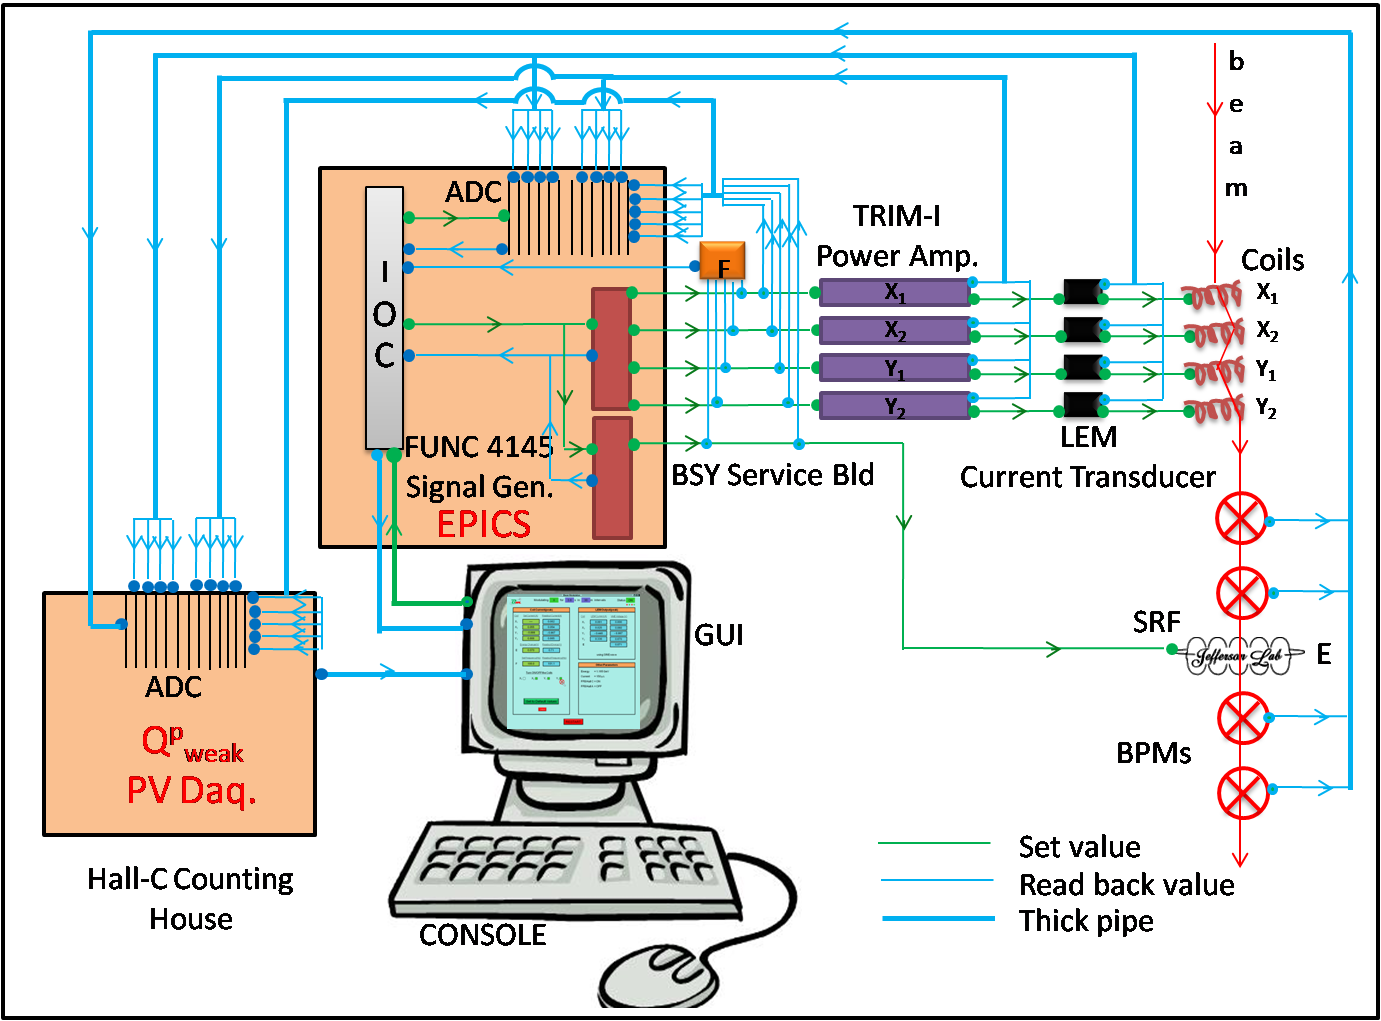
\includegraphics[width=14.5cm]{figures/bm_sketch}
%	\end{center}
%	\caption
%	[Beam modulation hardware sketch.]
%	{Beam modulation hardware sketch.}
%	\label{fig:bm_sketch}
%\end{figure}
%\end{singlespace}
%
%\subsection{Air-Core Coils}
%\label{Air-Core Coils}
%We plan to use JLab MAT(HF) air-core coils because they have sufficient field integral, they are readily available due to a recent switch of the FFB system to lower inductance coils, and they are short so can be easily tucked in almost anywhere.  Their properties have been measured and summarized in an Excel file by Sarin Philips (JLab). [ref: http://qweak.jlab.org/doc-public/ShowDocument?docid=979 ] The most critical parameters are summarized in Table 4. (For reference, the total impedance is $X_{tot}$ = 1.6 $\Omega$ + 2$\pi$f(0.0038H).)  S. Philips also determined the reduction in field due to the skin effect in a standard stainless steel beampipe to be roughly 10\% at 1 KHz, and less than a few percent at our nominal frequency of 250 Hz. The amplifiers we plan to use limit us to sinusoidal modulation at 250 Hz, so we will ignore the skin effect henceforth.
%
%
%\subsection{Coil Siting}
%\label{Coil Siting}
%The nomenclature we use is from the OPTIM deck found in Appendix II. As shown in Figure 5, our 1st coil is in drift oD7028, located just after quadruple 3C08 and before the dipole 3C05. The 2nd coil will be in drift 0D7031, after dipole 3C06 but before dipole 3C07. The separation is about 9.5 m. 
%Initially, we tried to put both coils into a single ~1m drift, but the angle kicks of interest required excessively high field integrals. Separating the coils by more than 1 meter requires straddling an active beam element. We decided to straddle two dipoles with no intervening quadrupoles. Not only does this seem natural in an OPTIM context (since the orbit inside a dipole is plotted effectively like a drift), but it would simplify any trigonometric calculations if we ever have to do any cross-checks. 
%
%\begin{singlespace}
%\begin{figure}[h]
%	\begin{center}
%	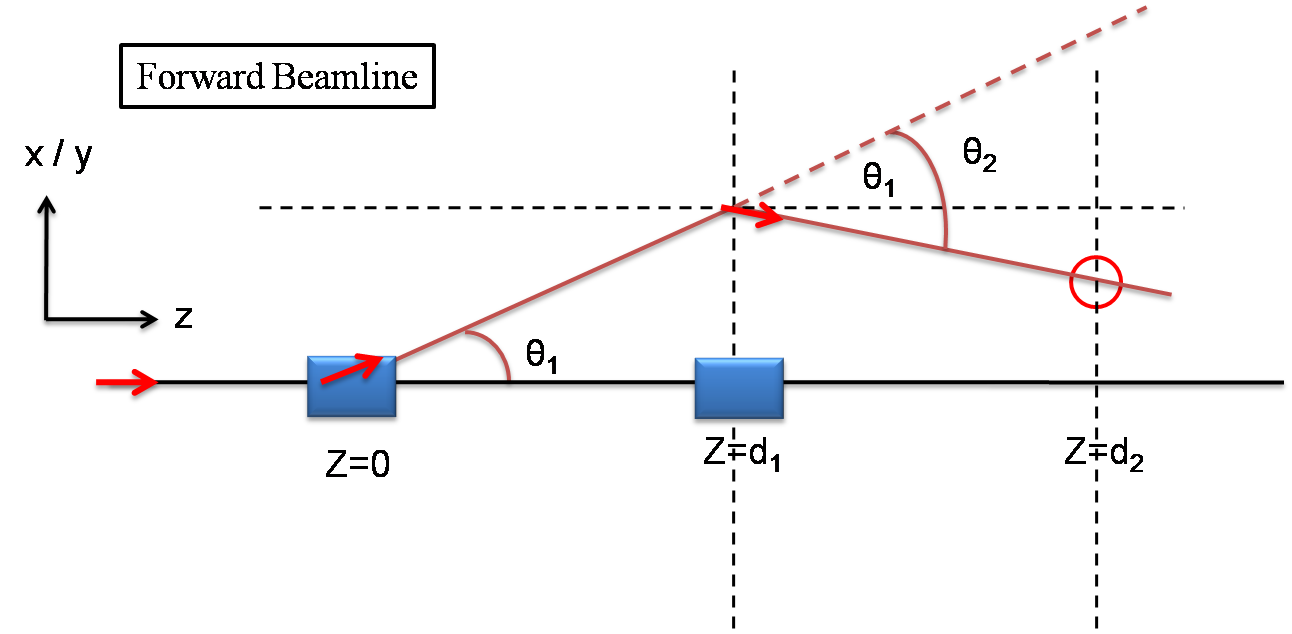
\includegraphics[width=14.5cm]{figures/bm_calc}
%	\end{center}
%	\caption
%	[Beam modulation sketch.]
%	{Beam modulation sketch.}
%	\label{fig:bm_calc}
%\end{figure}
%\end{singlespace}
%
%\subsection{Energy Modulation Hardware}
%\label{Energy Modulation Hardware}
%This procedure uses   an energy vernier of a cryo-module in South Linac of the accelerator. Every 1 hour of a production run, the procedure will begin what is called a supercycle for ~1 minute. Within each supercycle, modulation coil pair has its current ramped up and down with a proper ratio to each other. The final cycle of the supercycle is the modulation of the energy vernier. Each cycle can be programmed to be about 1minutes. The response of the beam position monitors and detectors can be measured. One of the standard features of the accelerator is the use of Fast Feedback (FFB) to maintain a steady beam position. 
%
%\section{Bench Tests}
%\label{Bench Tests}
%
%\begin{singlespace}
%\begin{table}
%\begin{center}
%  	\caption
%  	[Beam modulation bench test.]
%  	{Beam modulation bench test.}
%  \begin{tabular}{ l | c }
%%    \hline
%    \noalign{\hrule height 1pt}
%    	The Components & Quantity \\ 
%%    	\hline
%    \noalign{\hrule height 1pt}
%			Signal Generator & 1 \\
%			TRIM-II & 2 \\ 
%			MAT Coil & 2 \\ 
%			LEM & 1 \\
%			Ammeter & 2 \\
%			Power Supply & 1 \\
%			Tesla Meter & 1 \\ 
%%			\hline
%    \noalign{\hrule height 1pt}
%  	\end{tabular}
%  \label{bench_test}
%\end{center}
%\end{table}
%\end{singlespace}
%
%The Signal Generator generates SINE wave of different amplitude and frequency as the input voltage to the TRIM-II which is basically a power amplifier. The amplified signal goes to coil through a single LEM (current transducer) either in phase or out of phase from two coils. The currents through the coils are measured by ammeter. The Magnetic fields of the coils are measured by the Tesla Meter. We have done our measurements with MAT coil of length 10 cm long for several different frequencies. In the next section I am giving a brief of data taking.
%
%We did extensive bench testing with the proposed MAT(HF) coils and the TrimII amplifiers so that (except for the absence of long drive cables) we would be able to predict how the installed system would work. The TrimII amplifier was controlled via an analog input from a simple bench-top function generator (the ???). 
%
%
%\section{Waveform}
%
%\subsection{Waveform}
%\label{Waveform}
%The TrimII amplifier is unable to drive square or even triangular waveforms in the frequency range of interest. Satisfactory results were obtained only with sinusoidal waveforms. We would have preferred being able to generate at least square-ish modulation (similar to the square helicity reversal), but we are under budget and schedule pressure to use the existing TrimII amplifiers. 
%
%\subsection{Frequency Range}
%\label{Frequency Range}
%For a test range of 10H-500 Hz and nominal 3A (peak) output, we were able to reliably drive sinusoidal waveforms up to 250 Hz. At that frequency, the coil impedance becomes approximately Xtot= 1.6 ? + 2?f(0.0038H) = 7.6 ? so the amplifier has to provide 22.8 V (peak). The maximum output voltage of the TrimII amplifier appears to be approximately 
%+-27 V, but it isn't strictly bipolar due to the use of NPN diodes for one polarity and PNP diodes for the other. So while one could go a bit higher in frequency than 250 Hz, there would be a rapidly increasing risk of generating asymmetrical sine-like waves (and hence a small DC beam position offset). 
%
%\subsection{Maximum Current}
%\label{Maximum Current}
%With sustained operation, the coils become quite hot to the touch at Ipeak = 7.07 A (Irms = 5 A). This is significantly above Qweak's nominal maximum current Ipeak = 3 A, but it's worth discussing since future experiments at higher beam energy might try to push the envelope. Although measurements at 1\% duty factor would take only 36 seconds per hour, one must assume that a parity violation experiment will eventually take long, dedicated beam modulation runs. Unless cooling fans installed, damage to the enamel-insulated wires or any plastic components could result if Ipeak = 7.07 A is significantly exceeded. We haven't tried to determine the "smoke point", but bear in mind that P = R I2 so the temperature will increase rapidly with current above Ipeak = 7.07 A.  It is hopefully understood that Ipeak = 7.07 A refers to the peak current of a sinusoidal waveform, and NOT to a maximum DC current which would have a factor of 2 greater power dissipation!  
%
%\begin{enumerate}
%	\item measured the field integral with a GMW Hall Probe 
%	\item monitored the output waveform quality using a LEM current transducer 
%	\item drove two coils simultaneously from our FANUC VME function generator 
%\end{enumerate}
%
%WHAT DO WE DO ABOUT THE PROBLEM OF EXCESSIVELY SMALL CURRENTS FOR POSITION MODULATION????
%
%\section{OBSERVATIONS}
%\label{OBSERVATIONS}
%The TRIM II is not a linear device. It has frequency dependence. As we are going to higher frequencies starting from 10 Hz to 500 Hz, we are getting higher output voltages across the coils for same input voltage form signal generator with sine wave. As we are going to higher voltages for a fixed frequency, the TRIM II is showing non linearity also. Near the saturation current the TRIM II is getting locked by itself especially with higher frequency. 
%We are a getting a phase shift of 180� between the TRIM II output and the LEM current. 
%
%\section{EXTENSION TO OTHER JLAB PARITY VIOLATION EXPERIMENTS }
%\label{EXTENSION TO OTHER JLAB PARITY VIOLATION EXPERIMENTS}
%The system described in this report should be useful for other parity violation experiments such as the Moeller experiment at 11 GeV in Hall A. Some basic limitations should be kept in mind. First of all, the modulation amplitude of the system described here will scale like Ebeam(GeV)/1.165, hence the amplitudes at 11 GeV will be smaller by an order of magnitude. If the amplitude becomes smaller than the random beam jitter, convergence will be greatly slowed. The air-core coils can be driven harder if the duty factor is limited or if fans are used, but at about 5A (rms) they become hot enough to risk damaging the enamel coatings on the wires under continuous duty. Secondly, at the frequencies of interest, the coil is an almost purely inductive load, so the voltage needed to drive a given current is nearly proportional to frequency. If we wish to modulate the beam faster than the 250 Hz system described here, faster, higher voltage power amplifiers than the TrimII would be needed. Alternatively, larger field integrals could be obtained for a given current by replacing air-core coils with ferrite magnets. Finally, because the final quadrupole is closer to the target in the 1C line, it should be somewhat easier to generate a given angle kick at a given beam energy as compared to the 3C line. 
%
%\section{SUMMARY}
%\label{Summary}
%We have presented a design for sinusoidal modulation up to 250 Hz which is robust and well-suited for experiments measuring small parity violating asymmetries. At the cost of 1\% of our beamtime, we will be able to measure all sensitivities to 10\% accuracy each day.  The pairs of coils can be tuned to deliver relatively pure position or angle modulations, making it much less likely that one when encounter singular matrices when solving for the sensitivities.  If the design optics should change for any reason, we can simply change the ratio of coil currents without having to move coils. At 250 Hz and 1.165 GeV, our bench tests confirmed the TrimII power amplifier is able to provide the desired 50?m, 50 ?rad beam modulation amplitudes with existing air-core HF(MAT) coils. However, to provide similar amplitudes for the MoellerPV experiment at 12 GeV in Hall A may require an upgrade of the amplifier or magnets. 
%
%
%
%
%\begin{landscape}
%\subsubsection{Details1}
%Small changes in these parameters will create a change in rate which, if beam helicity dependent, would create a false asymmetry. While the source group tries to keep these helicity-correlated parameter changes as small as possible, the goal of our beam modulation group is to occasionally induce controlled beam parameter changes dXi, measure the resulting detector false asymmetry Aifalse, and determine the detector sensitivities Aifalse/dXi. This will allow later correction of beam false asymmetries via ACORRECTION = i=1,5 (Aifalse/dXi)? Xi.  Even if these corrections prove to be small under ideal running conditions, the modulation system described here will allow us to quickly determine if undesirable changes have occurred. ~\cite{arr98}
%
%\begin{equation} \label{equ:nucltransp}
%T = 
%{\left( \frac{\bar Y}{\bar Y_{\rm MC}} \right)_A}/
%{\left( \frac{\bar Y}{\bar Y_{\rm MC}} \right)_{\rm D}},
%\end{equation}
%\end{landscape}
%
%\section{Simulation}
%
%\subsection{OPTIM}
%\label{OPTIM}
%We used a software, OPTIM, to do basic calculation for beam modulation. OPTIM is basically computer code for linear and non-linear optics calculations \cite{website:optim}. Main OPTIM deq. file contain all the detailed information about all the beamline elements. It has the information like location of the beamline, field strength, size, orientation etc. One can also get the transfer matrices between any two beamlime elements using the software. It also produces simulated trajectories through the beamline from one element to another. We used OPTIM to give us simulated trajectories form beam modulation magnet pair at the beginning of Hall-C beamline to the Q-weak target. We also changed our basis of calculation from beam modulation coil co-ordinate to Q-weak target co-ordinate using OPTIM.
%
%
%%\begin{math}
%%\bordermatrix{&a_1&a_2&...&a_n\cr
%%          b_1 & 1.2  & 3.3  & 5.1  & 2.8  \cr
%%          c_1 & 4.7  & 7.8  & 2.4  & 1.9  \cr
%%          ... & ...  & ...  & ...  & ...  \cr
%%          z_1 & 8.0  & 9.9  & 0.9  & 9.99  \cr}
%%\end{math}
%%
%%
%%$3 \times 3$~Matrix:
%%
%%\[ \left( \begin{array}{ccc}
%%a & b & c \\
%%d & e & f \\
%%g & h & i \end{array} \right)\] 
%%
%%$3 \times 3$~Determinant:
%%
%%\[ 
%%\left[ \begin{array}{ccc}
%%\lambda - a & -b & -c \\
%%-d & \lambda - e & -f \\
%%-g & -h & \lambda - i \end{array} \right] = 
%%\left[ \begin{array}{ccc}
%%\lambda - a & -b & -c \\
%%-d & \lambda - e & -f \\
%%-g & -h & \lambda - i \end{array} \right]
%%\left[ \begin{array}{c}
%%\lambda - a \\
%%-d \\
%%-g \end{array} \right]
%%\] 
%%
%%\begin{center}
%%\framebox[\frameboxsize][c]{Systematic error due to regression schemes dependence is $\sim$ 0.0046 ppm.}
%%\end{center}
%%
%%\begin{Verbatim}[frame=single,
%%framerule=1mm,framesep=3mm,
%%rulecolor=\color{red},
%%fillcolor=\color{yellow}]
%%Verbatim line.
%%\end{Verbatim}
%%
%%org\textasciitilde nur
%%
%%\degrees{90}
%%
%%
%%\begin{figure}[!htb]
%%  \begin{center}
%%  \begin{tabular}{cccccccccccccccc}
%%    \begin{fmffile}{virtualTop1}
%%      \fmfframe(1,7)(1,7){
%%       \begin{fmfgraph*}(110,62)
%%        \fmfleft{i1}
%%        \fmfright{o1}
%%        \fmf{boson,tension=2}{i1,v1}
%%        \fmf{fermion,left=0.8,label=$t$}{v1,v2}
%%        \fmf{fermion,left=0.8,label=$\bar{b}$}{v2,v1}
%%        \fmf{boson,tension=2}{v2,o1}
%%        \fmflabel{$W$}{i1}
%%        \fmflabel{$W$}{o1}
%%       \end{fmfgraph*}
%%      }
%%    \end{fmffile}
%%   \end{tabular}
%%   \end{center}
%%   \caption{The caption.}
%%   \label{fig:feynGraph1}
%% \end{figure}


\begin{singlespace}
\begin{table}
\begin{center}
  	\caption
%  	[Beam modulation bench test.]
  	{The components of beam modulation bench test.}
  \begin{tabular}{ l | c }
%    \hline
    \noalign{\hrule height 1pt}
    	The Components & Quantity \\ 
%    	\hline
    \noalign{\hrule height 1pt}
			Signal Generator & 1 \\
			TRIM-II & 2 \\ 
			MAT Coil & 2 \\ 
			LEM & 1 \\
			Ammeter & 2 \\
			Power Supply & 1 \\
			Tesla Meter & 1 \\ 
%			\hline
    \noalign{\hrule height 1pt}
  	\end{tabular}
  \label{bench_test}
\end{center}
\end{table}
\end{singlespace}
 

\begin{singlespace}
\begin{figure}[!h]
	\begin{center}
	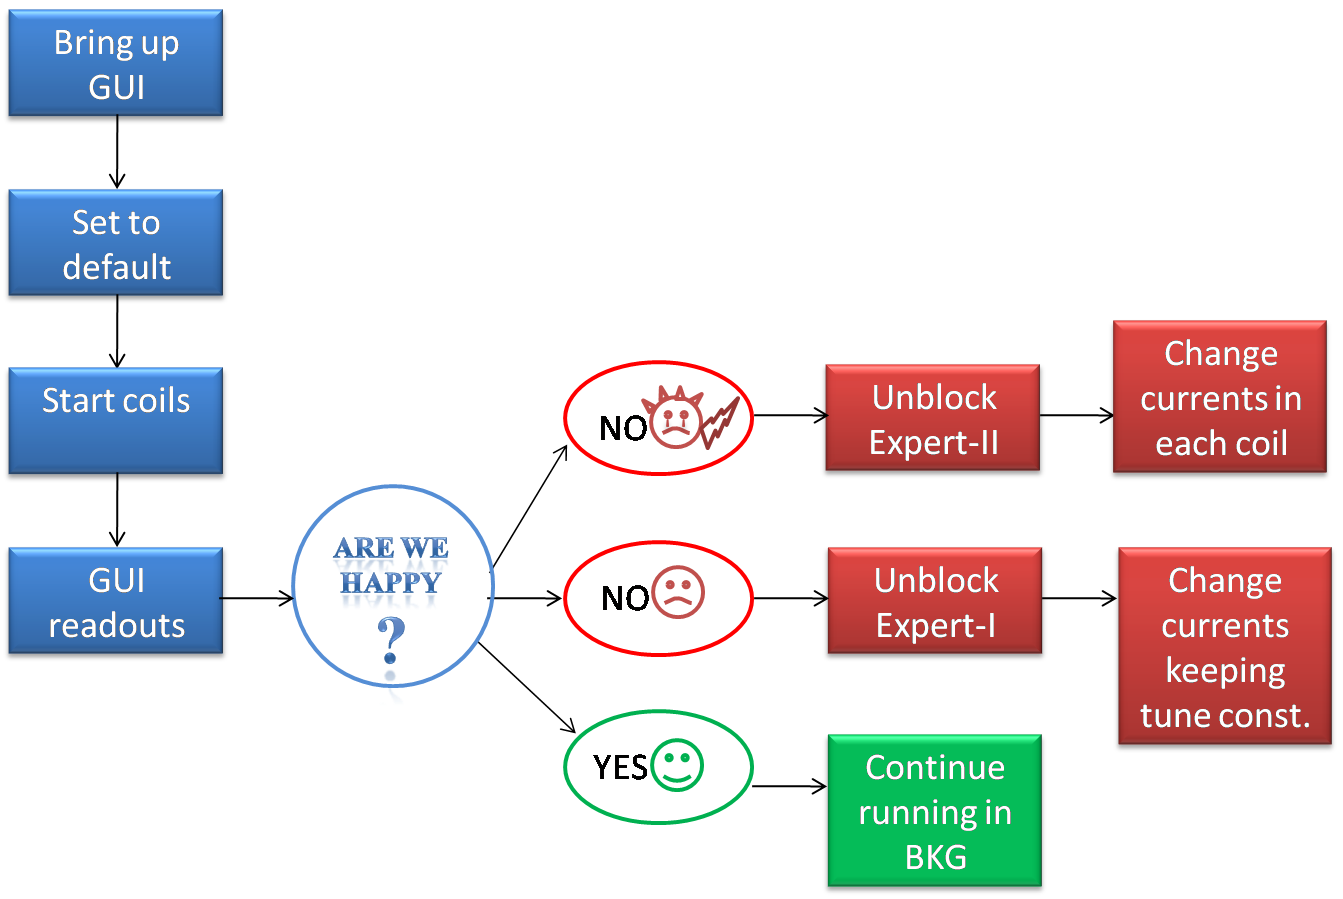
\includegraphics[width=15.0cm]{figures/BModGUI_FlowChart}
	\end{center}
	\caption
%	[BMod GUI design flow chart.]
	{BMod GUI design flow chart.}
	\label{fig:BModGUI_FlowChart}
\end{figure}
\end{singlespace}

\begin{singlespace}
\begin{figure}[!h]
	\begin{center}
	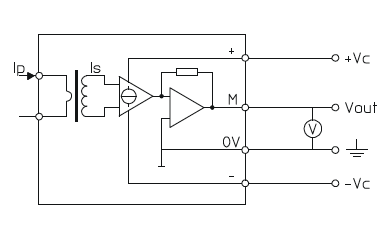
\includegraphics[width=15.0cm]{figures/BModCktLEM}
	\end{center}
	\caption
%	[BMod LEM current transducer circuit design.]
	{The circuit design of the LEM current transducer used to measure the current through the beam modulation magnet.}
	\label{fig:BModCktLEM}
\end{figure}
\end{singlespace}

\begin{singlespace}
\begin{figure}[!h]
	\begin{center}
	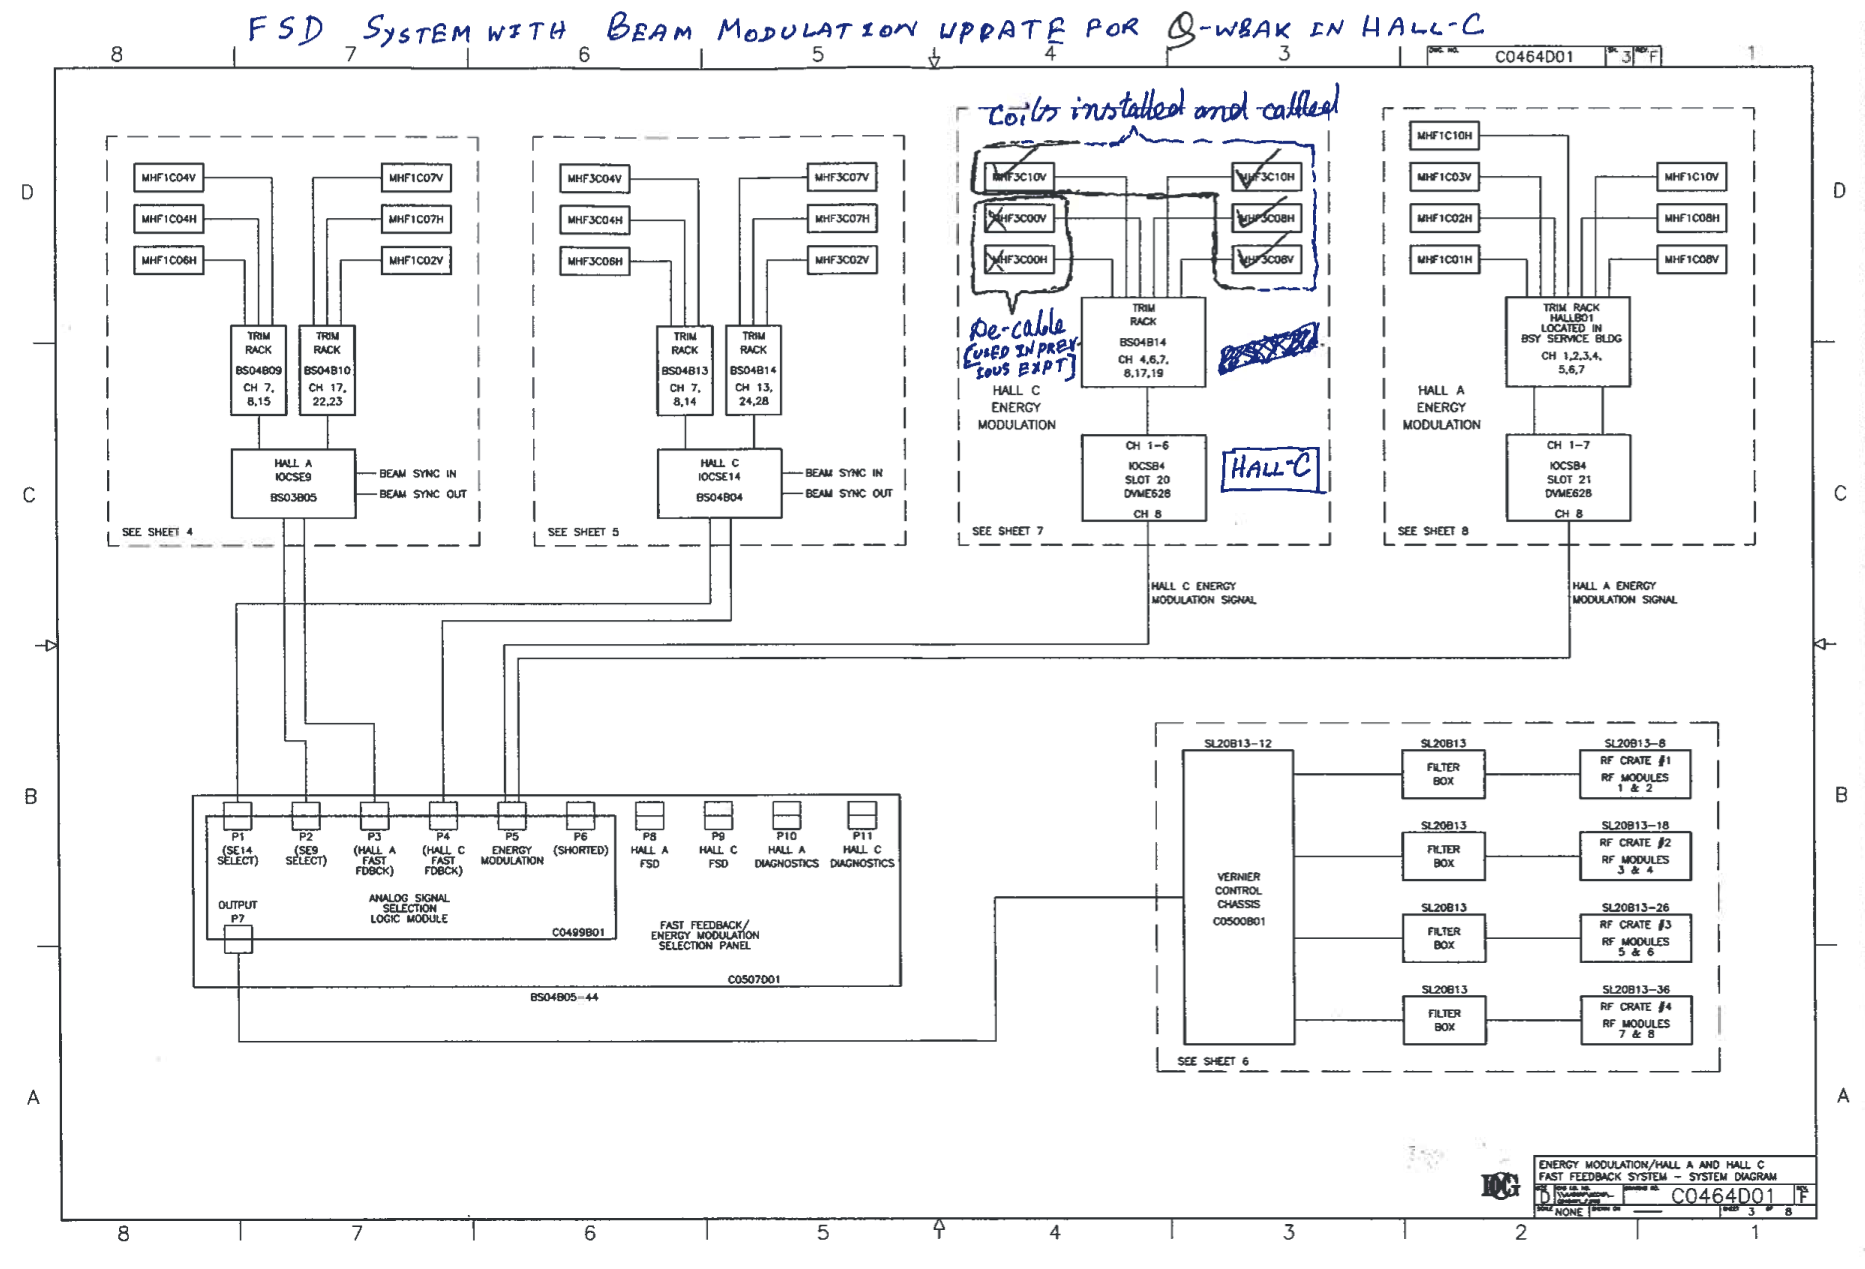
\includegraphics[width=15.0cm]{figures/FSD_correction}
	\end{center}
	\caption
%	[Fast shut down circuit diagram for Q-weak.]
	{Fast shut down circuit diagram for Q-weak. The modification shown are implemented before the experiment. }
	\label{fig:FSD_correction}
\end{figure}
\end{singlespace}



\begin{singlespace}
\begin{figure}[!h]
	\begin{center}
	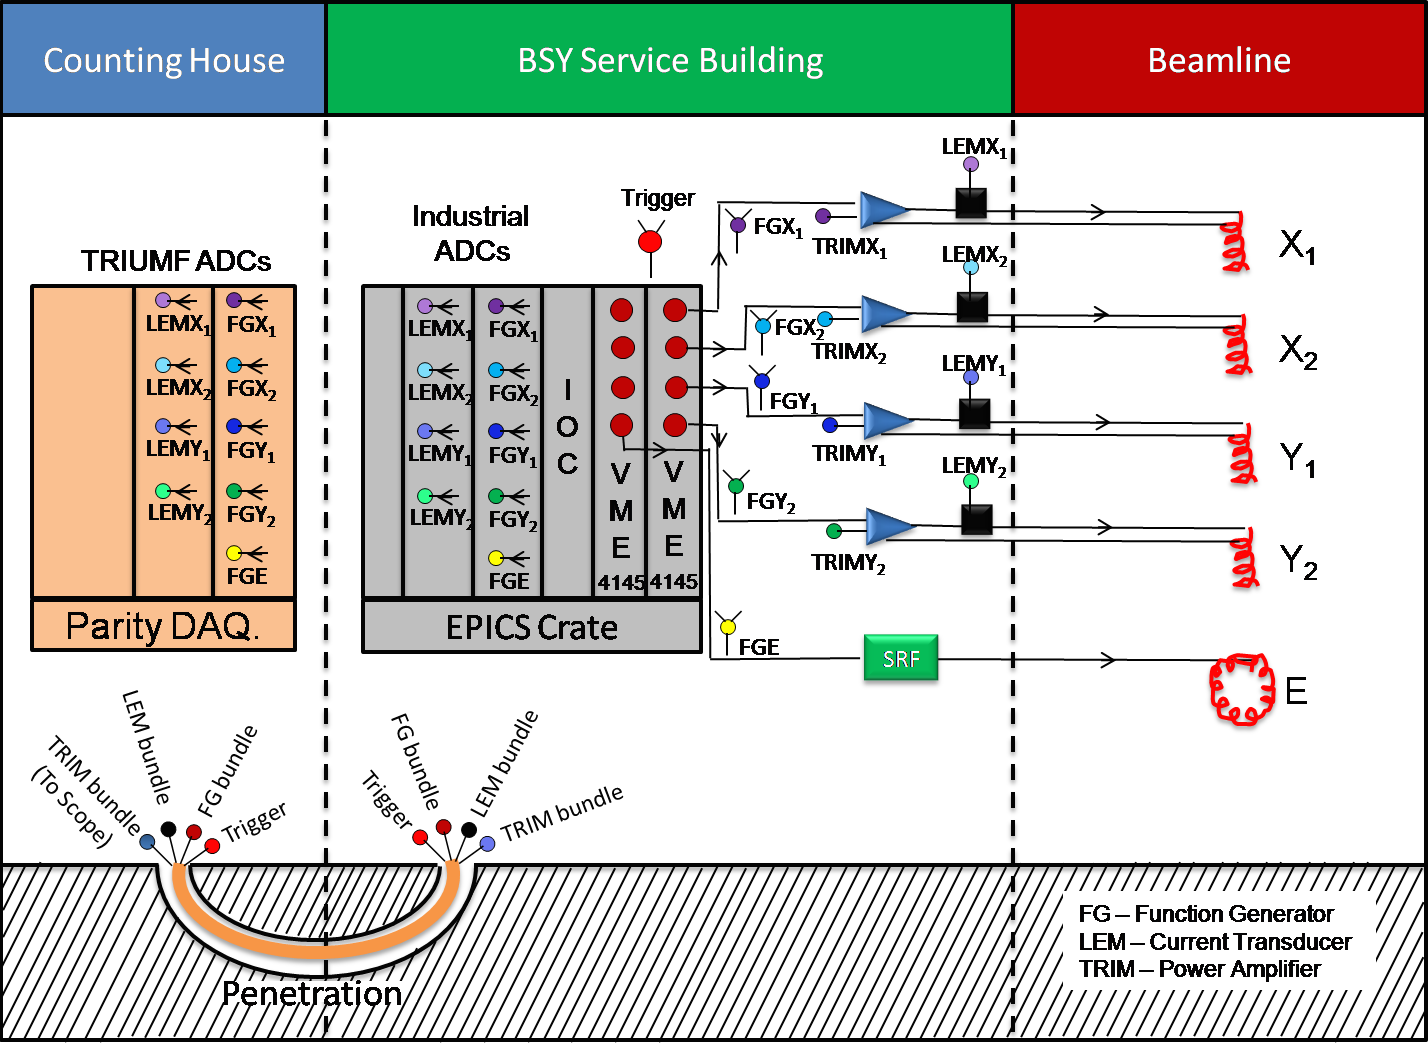
\includegraphics[width=15.0cm]{figures/BModCable}
	\end{center}
	\caption
%	[BMod cable.]
	{The cable path for the modulation system. The components are spanned into counting house Hall-C and beamline.}
	\label{fig:BModCable}
\end{figure}
\end{singlespace}

\begin{singlespace}
\begin{figure}[!h]
	\begin{center}
	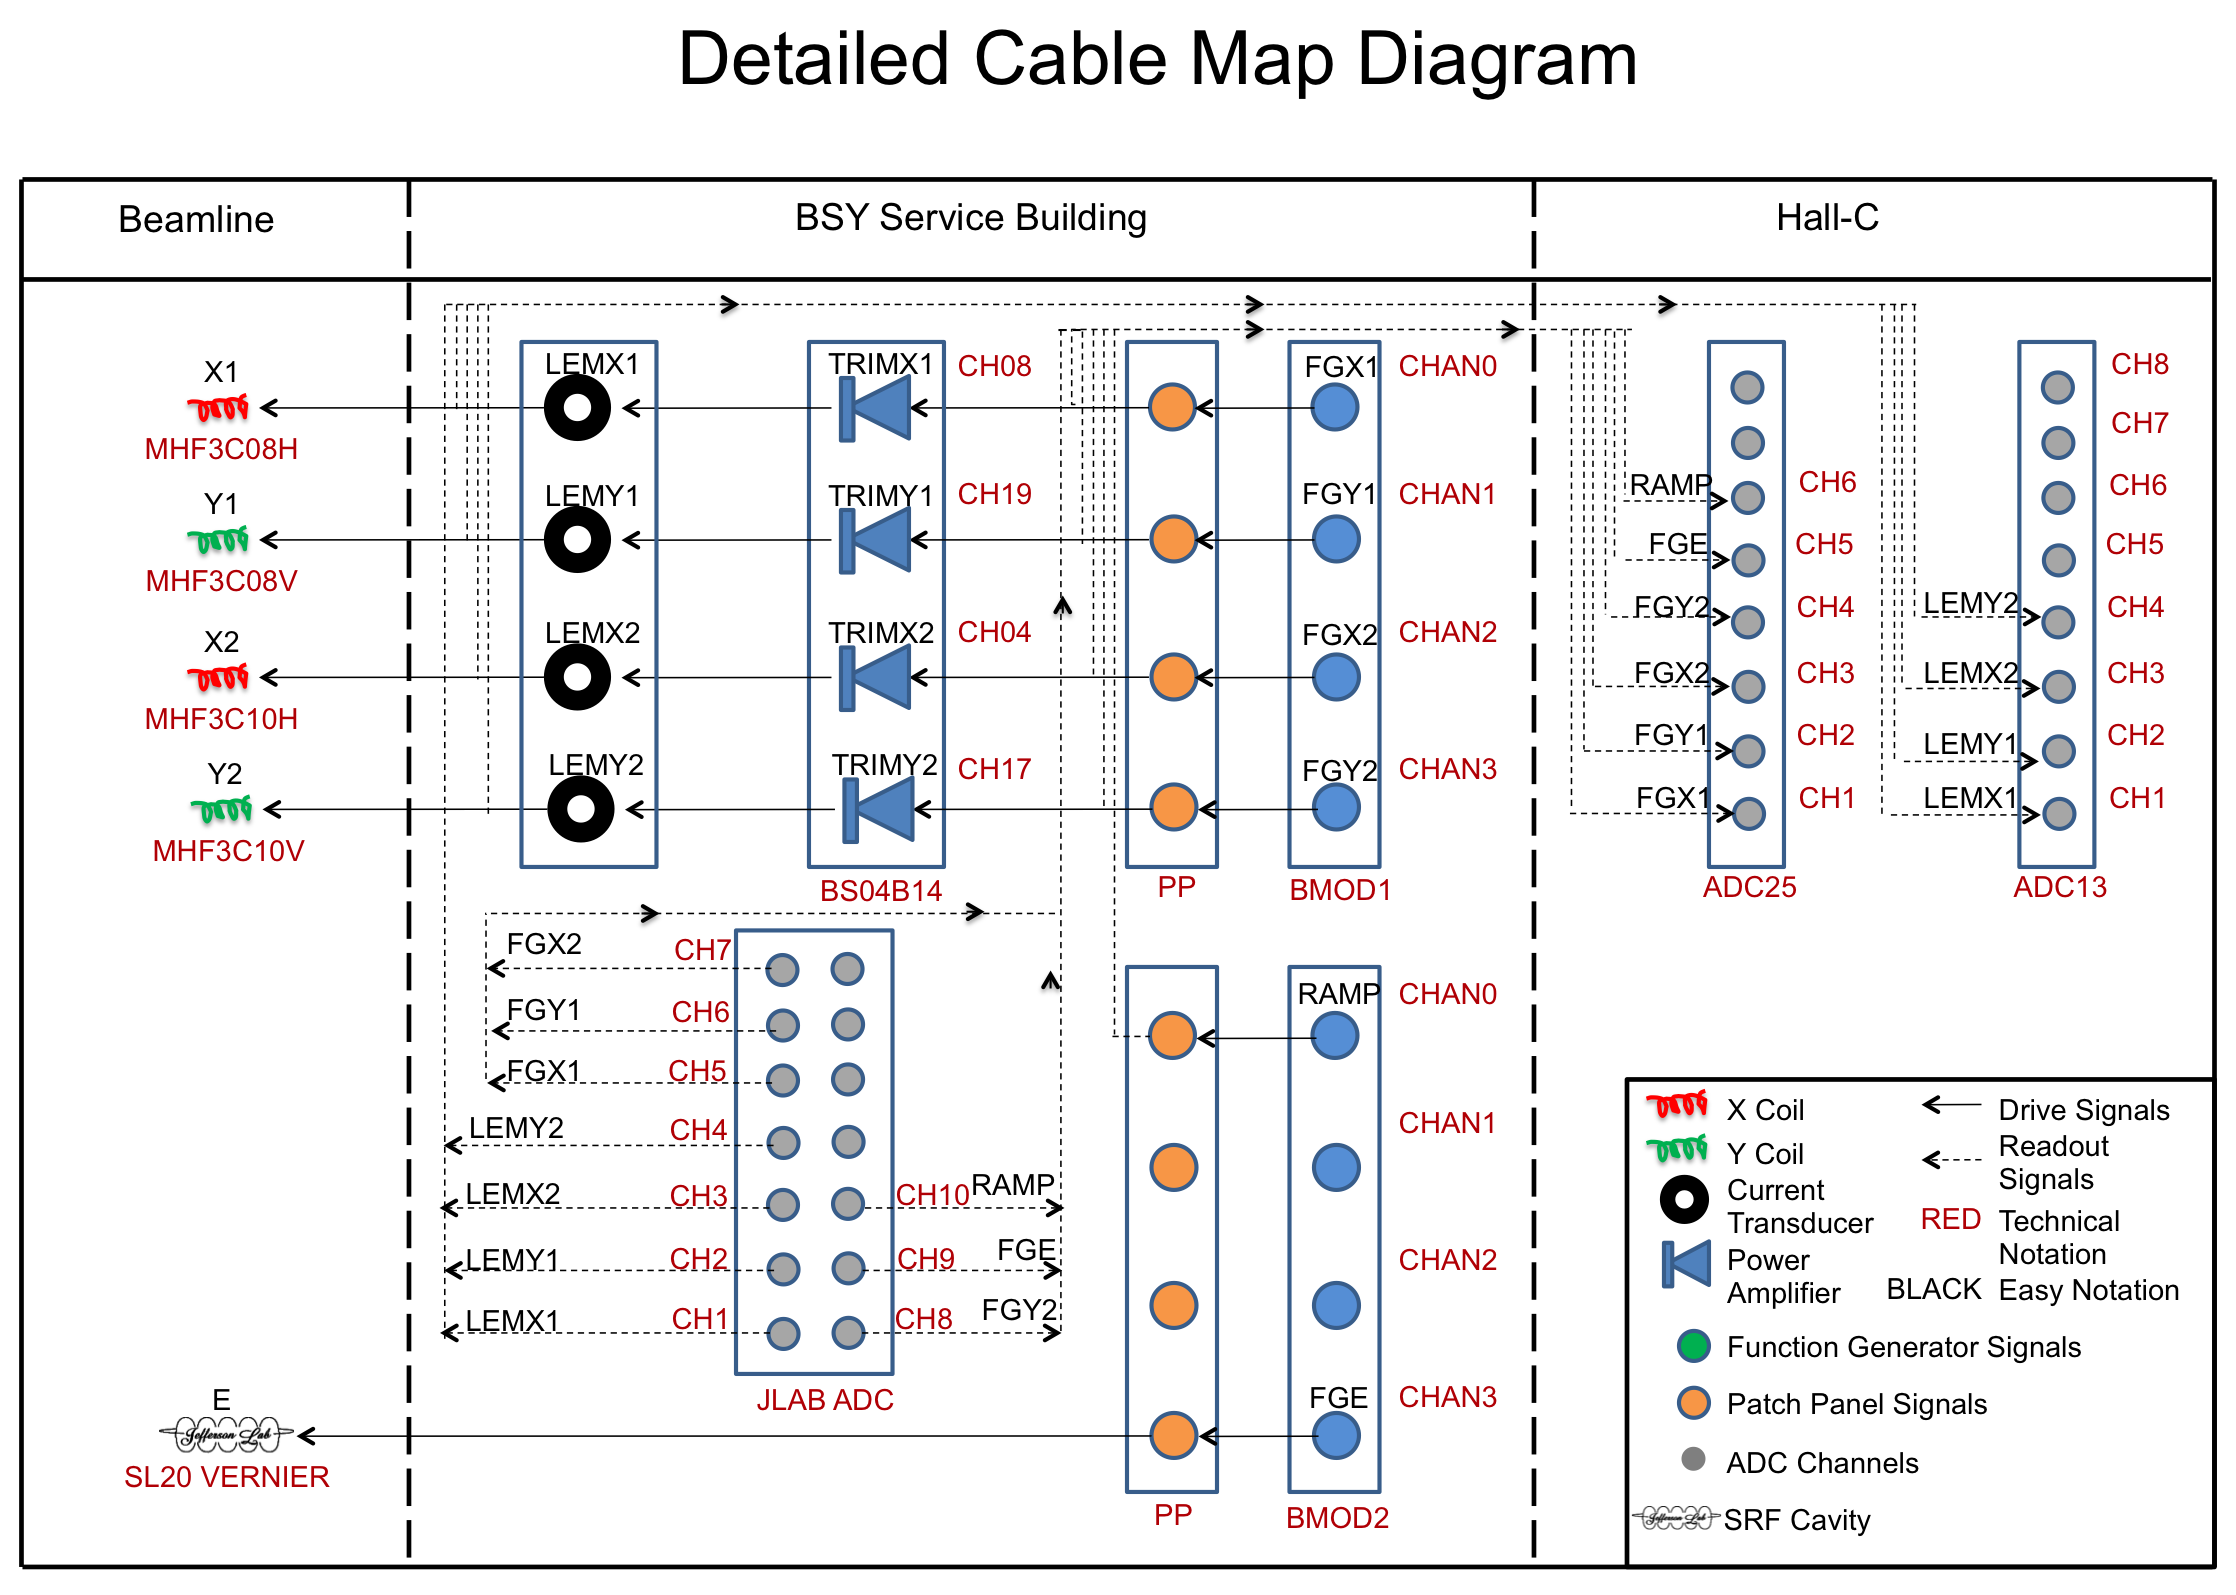
\includegraphics[width=15.0cm]{figures/BModCableMapDiagram}
	\end{center}
	\caption
%	[BMod cable map diagram.]
	{The cable map for the modulation system.}
	\label{fig:BModCableMapDiagram}
\end{figure}
\end{singlespace}


\begin{singlespace}
\begin{figure}[!h]
	\begin{center}
	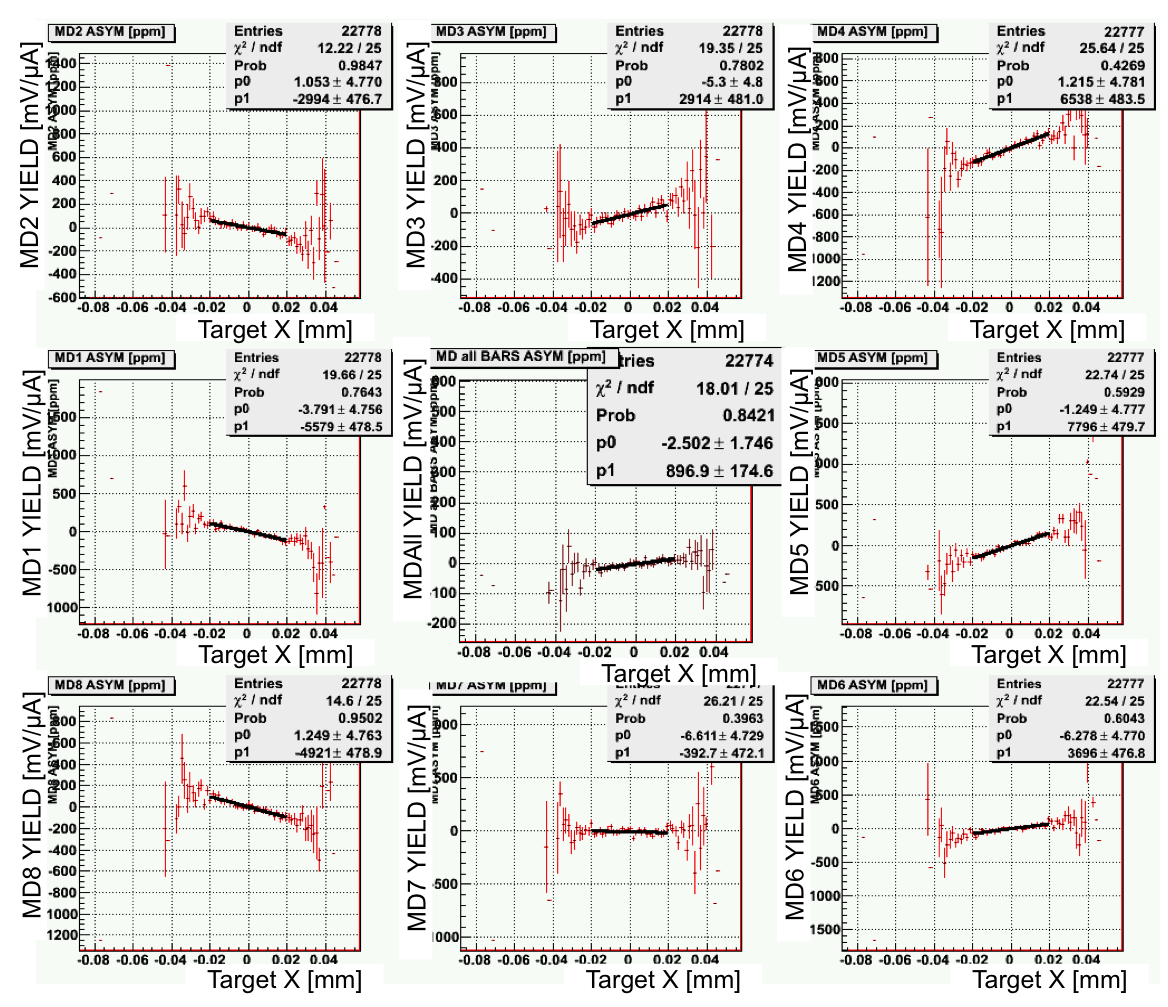
\includegraphics[width=15.0cm]{figures/NaturalJitterDetectorSensitivity}
	\end{center}
	\caption
%	[Main detector sensitivities with respect to target BPM X position for X modulation.]
	{Main detector sensitivities with respect to target BPM X position for X modulation. The eight octants along with combined sensitivities are shown. }
	\label{fig:NaturalJitterDetectorSensitivity}
\end{figure}
\end{singlespace}



\begin{singlespace}
\begin{figure}[!h]
	\begin{center}
	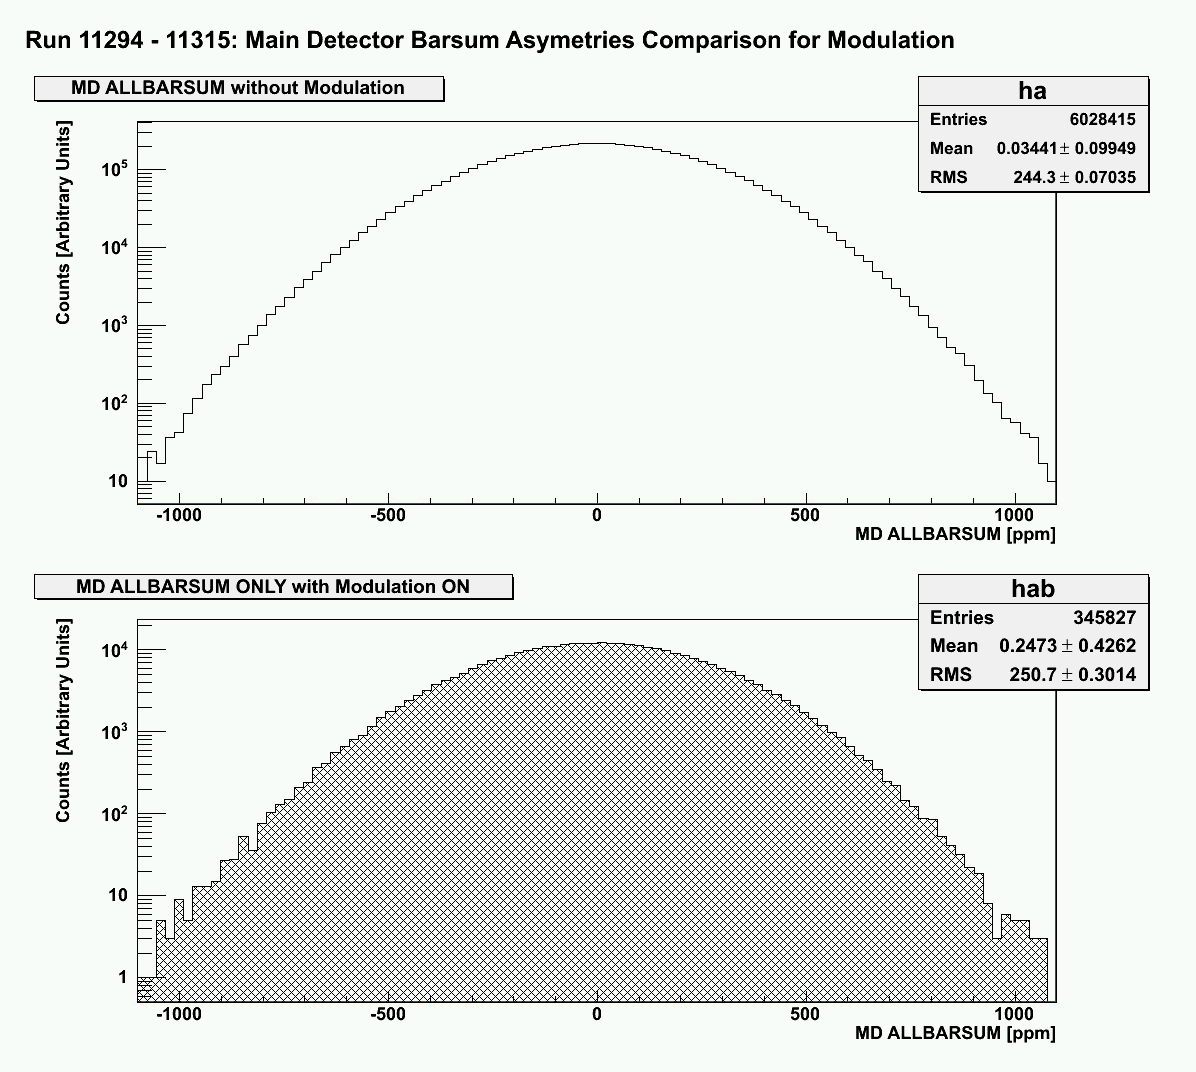
\includegraphics[width=15.0cm]{figures/BModEffectsMDAsyms}
	\end{center}
	\caption
%	[Effect of beam modulation on main detector asymmetry.]
	{Effect of beam modulation on main detector asymmetry. Comparison of main detector asymmetry when modulation is OFF (top) and modulation is ON (bottom) are shown here.}
	\label{fig:BModEffectsMDAsyms}
\end{figure}
\end{singlespace}

\begin{singlespace}
\begin{figure}[!h]
	\begin{center}
	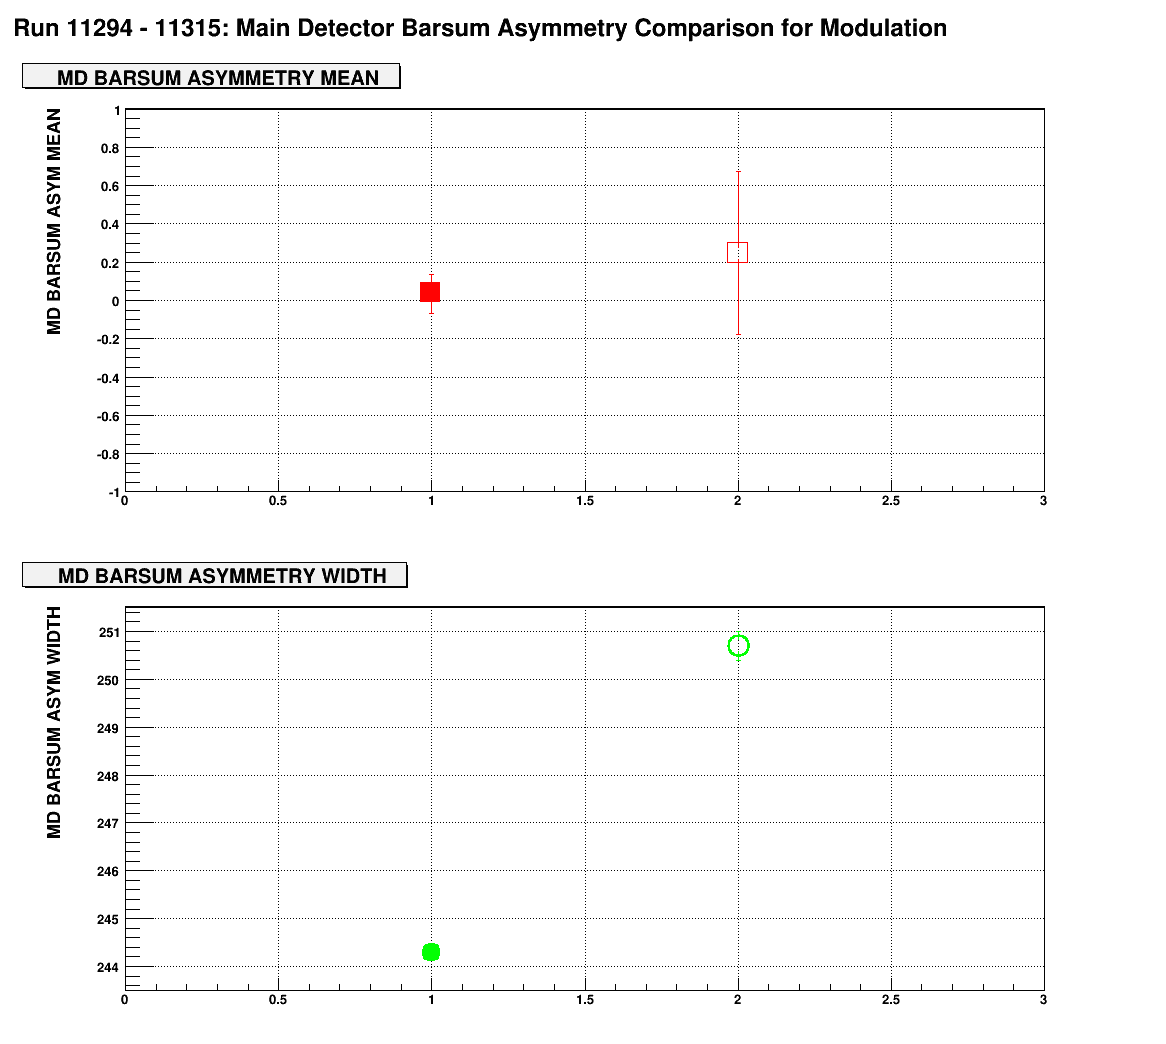
\includegraphics[width=15.0cm]{figures/BModEffectsMDCompare}
	\end{center}
	\caption
%	[Effect of beam modulation on main detector asymmetry.]
	{Effect of beam modulation on main detector asymmetry. Main detector asymmetry mean when modulation is OFF and ON (top) and asymmetry width (bottom) are compared here.}
	\label{fig:BModEffectsMDCompare}
\end{figure}
\end{singlespace}

\begin{singlespace}
\begin{figure}[!h]
	\begin{center}
	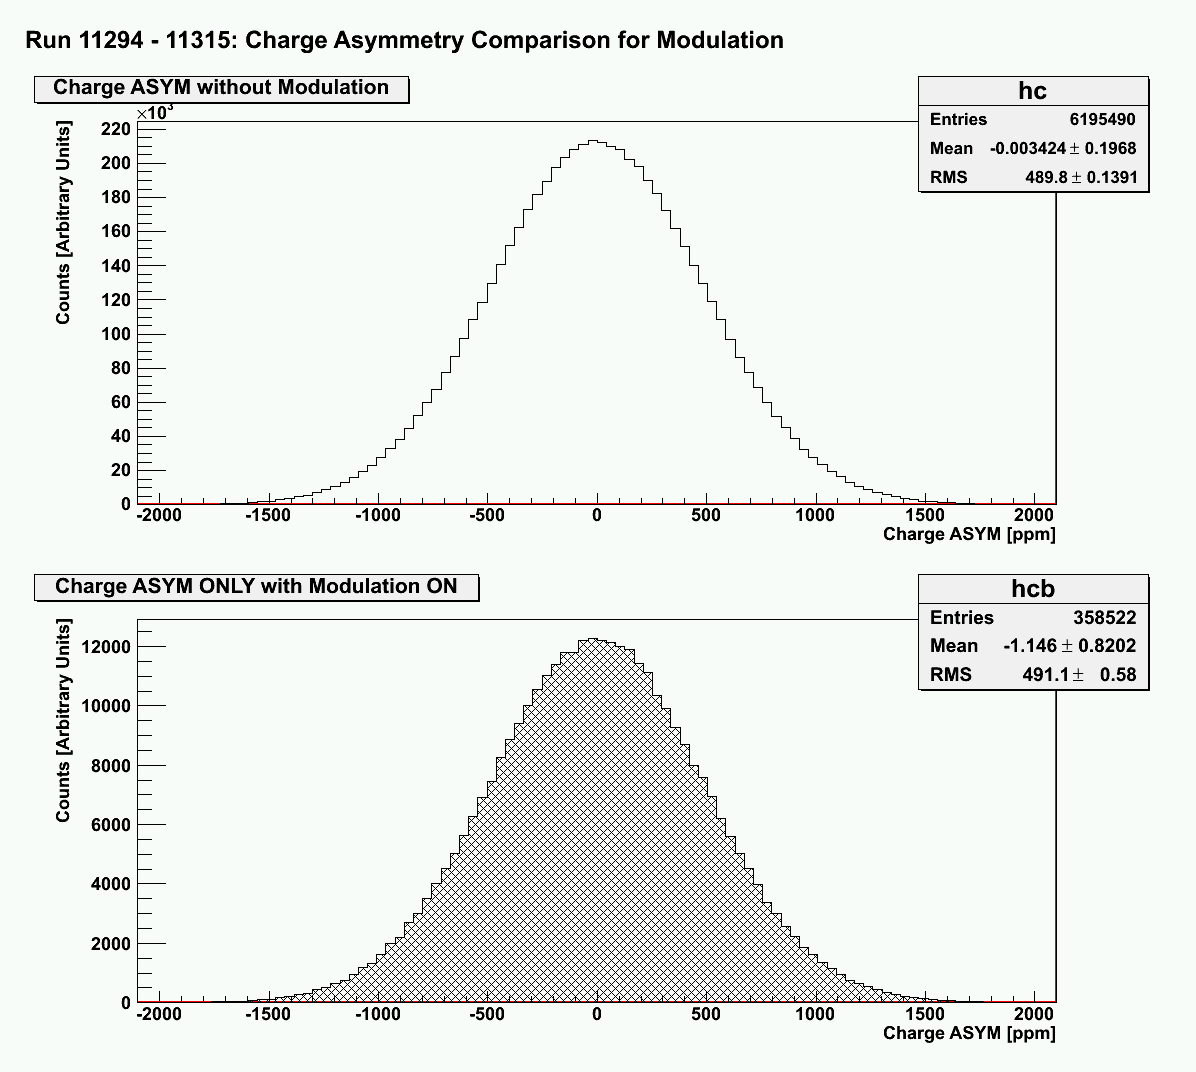
\includegraphics[width=15.0cm]{figures/BModEffectsChargeAsym}
	\end{center}
	\caption
%	[Effect of beam modulation on charge asymmetry.]
	{Effect of beam modulation on charge asymmetry. Comparison of charge asymmetry when modulation is OFF (top) and modulation is ON (bottom) are shown here.}
	\label{fig:BModEffectsChargeAsym}
\end{figure}
\end{singlespace}

\begin{singlespace}
\begin{figure}[!h]
	\begin{center}
	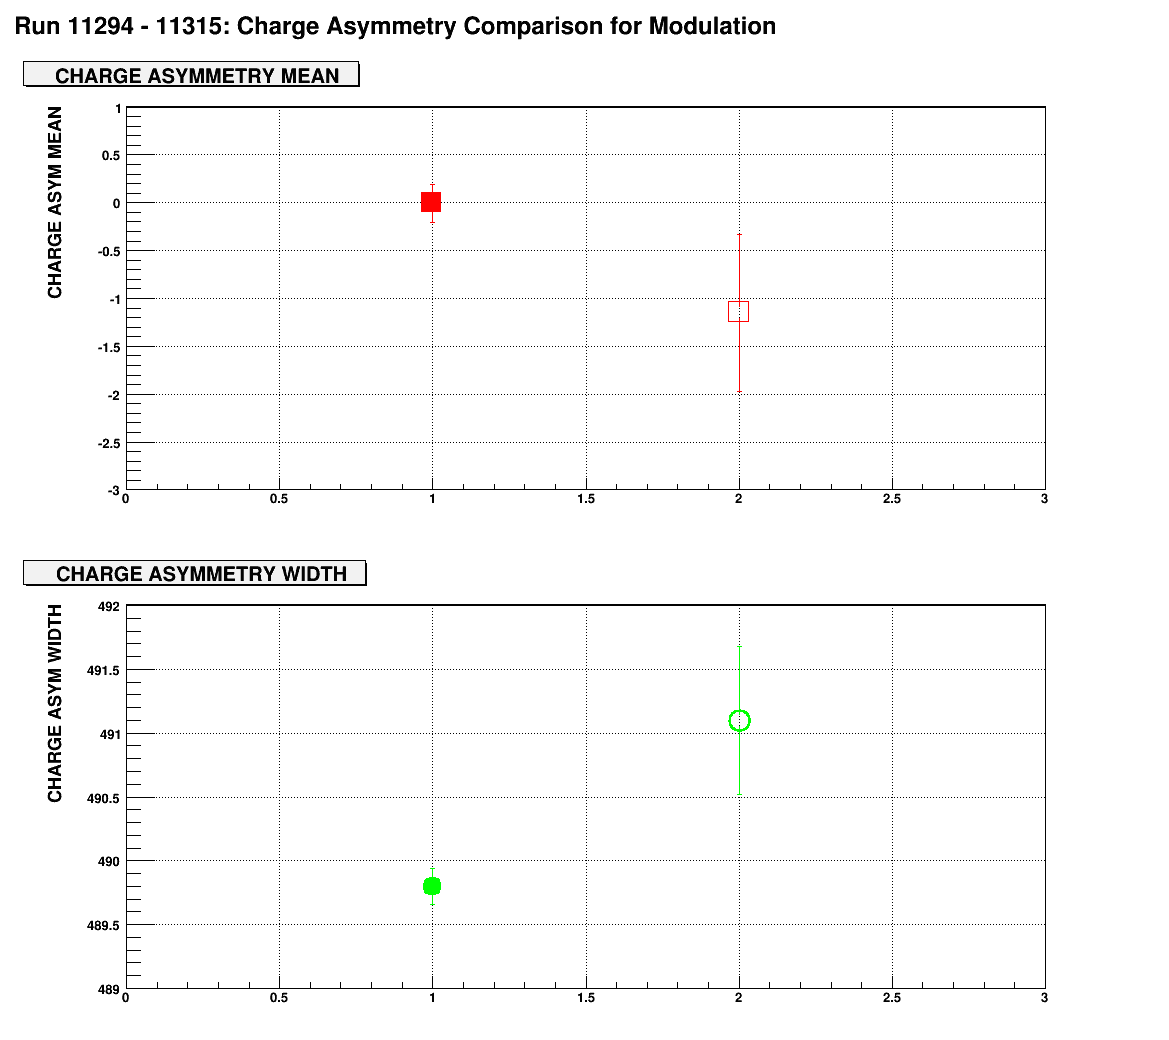
\includegraphics[width=15.0cm]{figures/BModEffectsChargeCompare}
	\end{center}
	\caption
%	[Effect of beam modulation on charge asymmetry.]
	{Effect of beam modulation on charge asymmetry. Comparison of charge asymmetry without modulation with charge asymmetry only during modulation ON.}
	\label{fig:BModEffectsChargeCompare}
\end{figure}
\end{singlespace}

\begin{singlespace}
\begin{figure}[!h]
	\begin{center}
	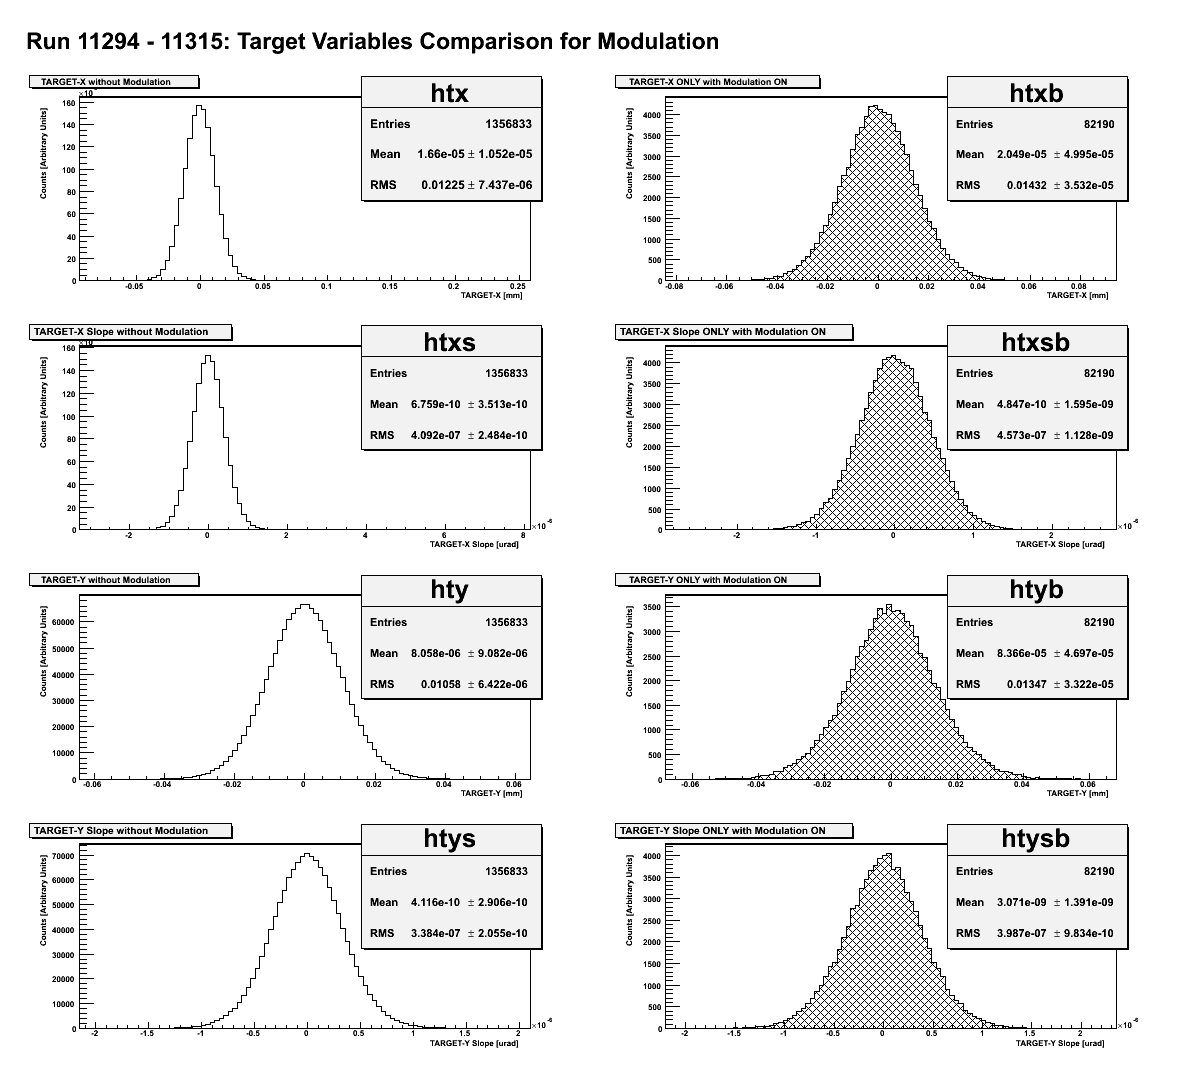
\includegraphics[width=15.0cm]{figures/BModEffectsTarget}
	\end{center}
	\caption
%	[Effect of beam modulation on target BPM.]
	{Effect of beam modulation on target BPM. Comparison of target BPM differences when modulation is OFF (left) and modulation is ON (right) are shown here. }
	\label{fig:BModEffectsTarget}
\end{figure}
\end{singlespace}



%\section{Beamline Drawing}

\begin{singlespace}
\begin{figure}[!h]
	\begin{center}
	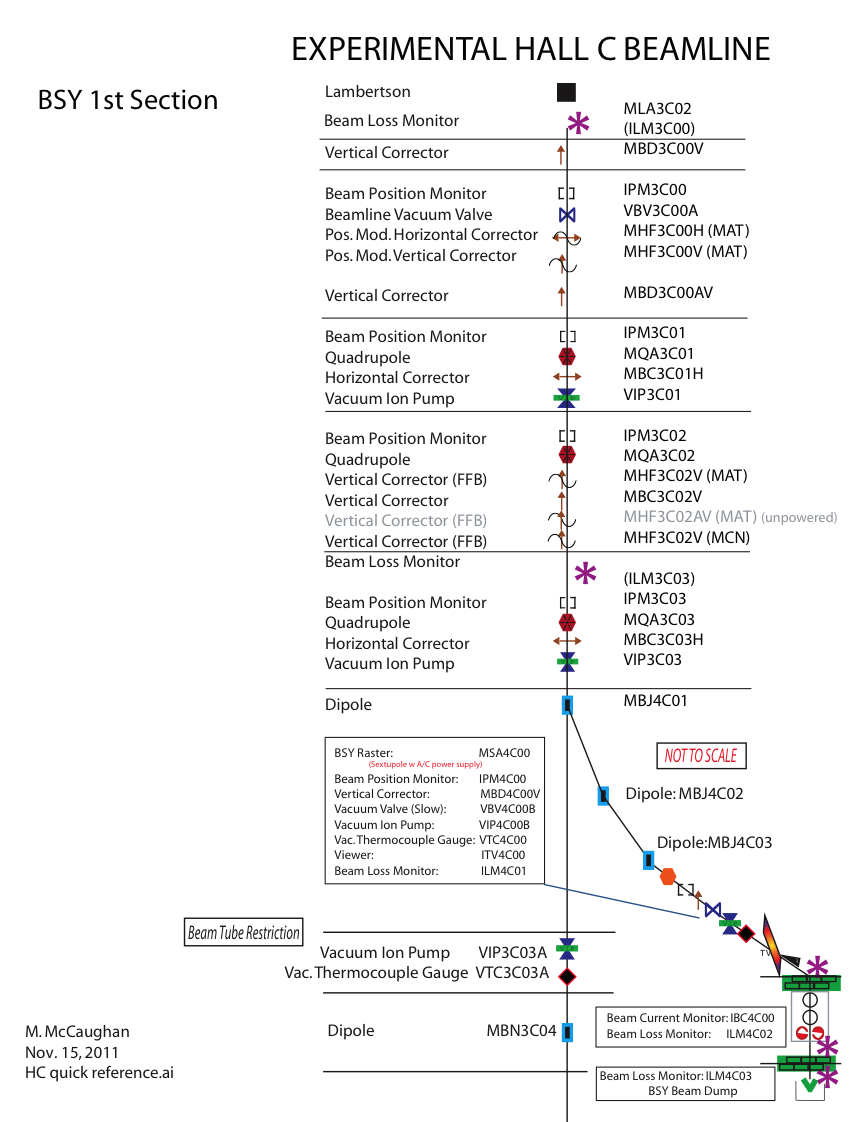
\includegraphics[width=15.0cm]{figures/BeamlineDrawing1}
	\end{center}
	\caption
%	[BeamlineDrawing1.]	
	{Beamline drawing 1.}
	\label{fig:BeamlineDrawing1}
\end{figure}
\end{singlespace}

\begin{singlespace}
\begin{figure}[!h]
	\begin{center}
	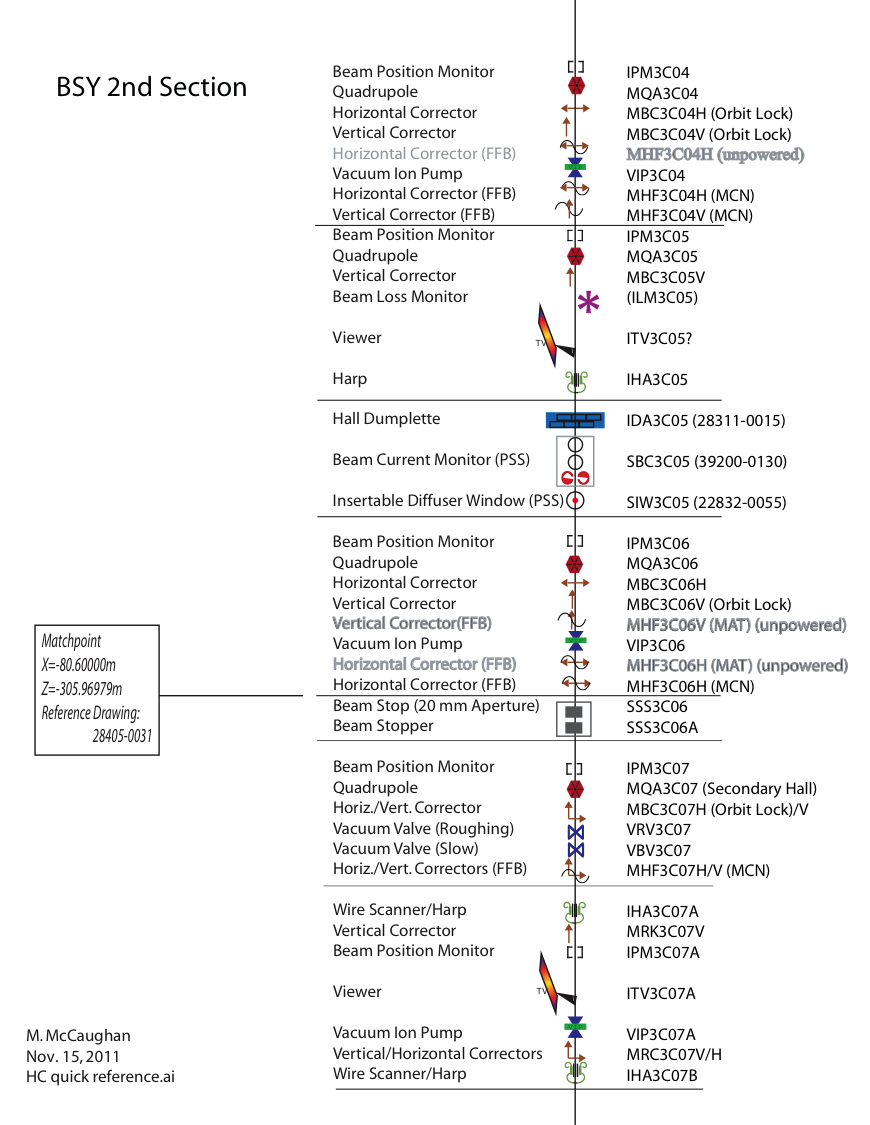
\includegraphics[width=15.0cm]{figures/BeamlineDrawing2}
	\end{center}
	\caption
%	[BeamlineDrawing2.]	
	{Beamline drawing 2.}
	\label{fig:BeamlineDrawing2}
\end{figure}
\end{singlespace}

\begin{singlespace}
\begin{figure}[!h]
	\begin{center}
	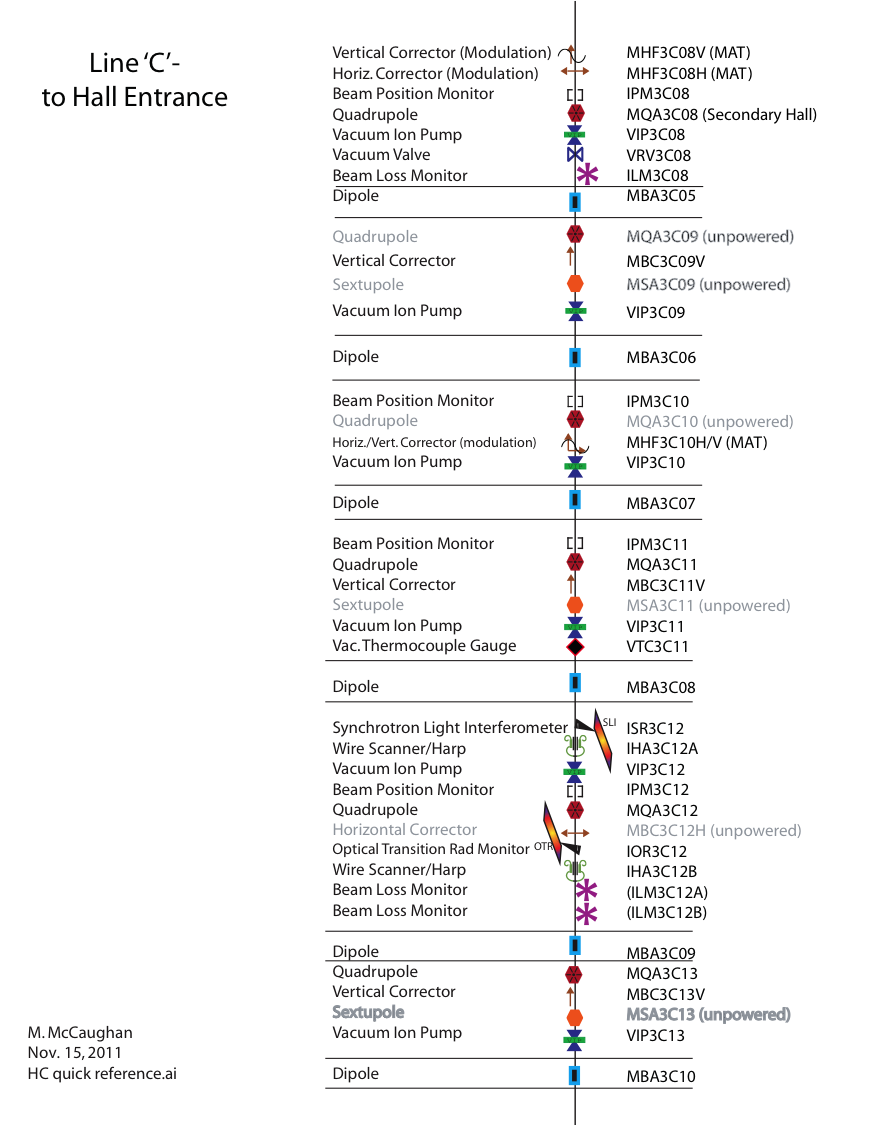
\includegraphics[width=15.0cm]{figures/BeamlineDrawing3}
	\end{center}
	\caption
%	[BeamlineDrawing3.]	
	{Beamline drawing 3.}
	\label{fig:BeamlineDrawing3}
\end{figure}
\end{singlespace}

\begin{singlespace}
\begin{figure}[!h]
	\begin{center}
	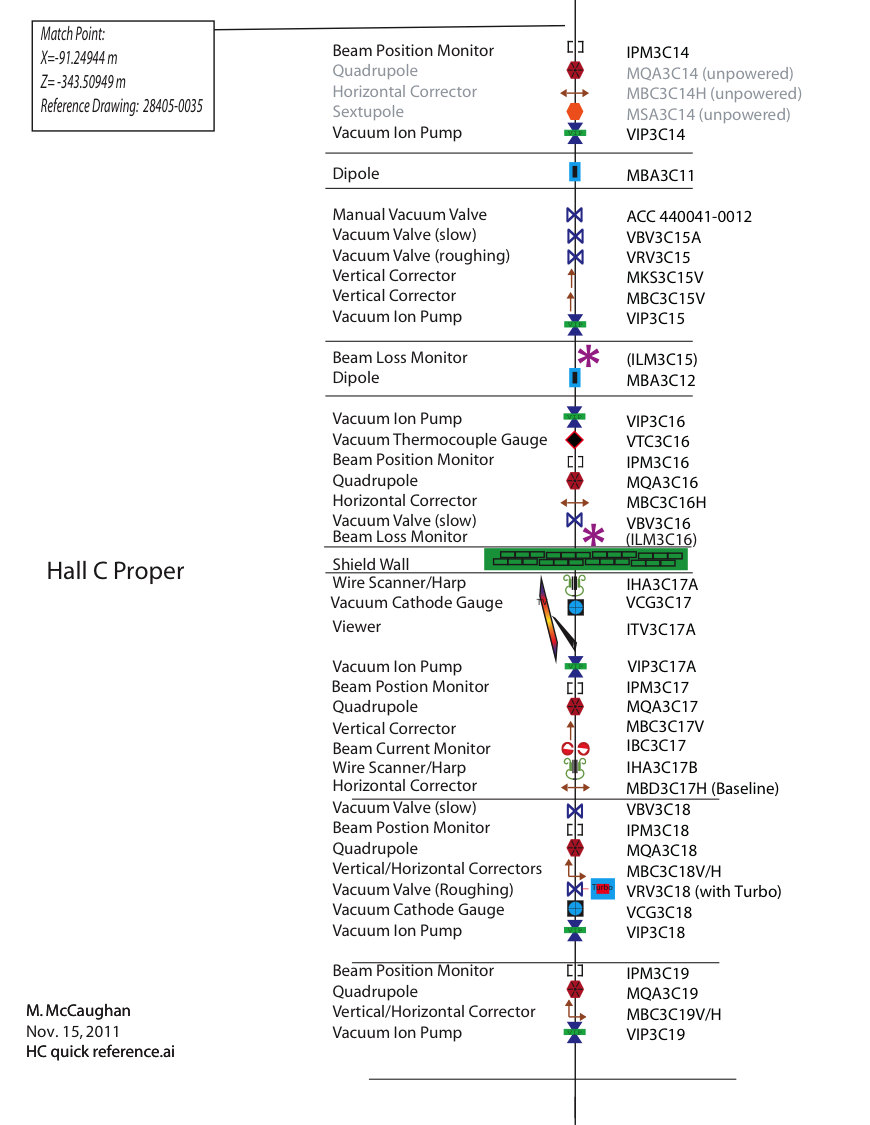
\includegraphics[width=15.0cm]{figures/BeamlineDrawing4}
	\end{center}
	\caption
%	[BeamlineDrawing4.]	
	{Beamline drawing 4.}
	\label{fig:BeamlineDrawing4}
\end{figure}
\end{singlespace}

\begin{singlespace}
\begin{figure}[!h]
	\begin{center}
	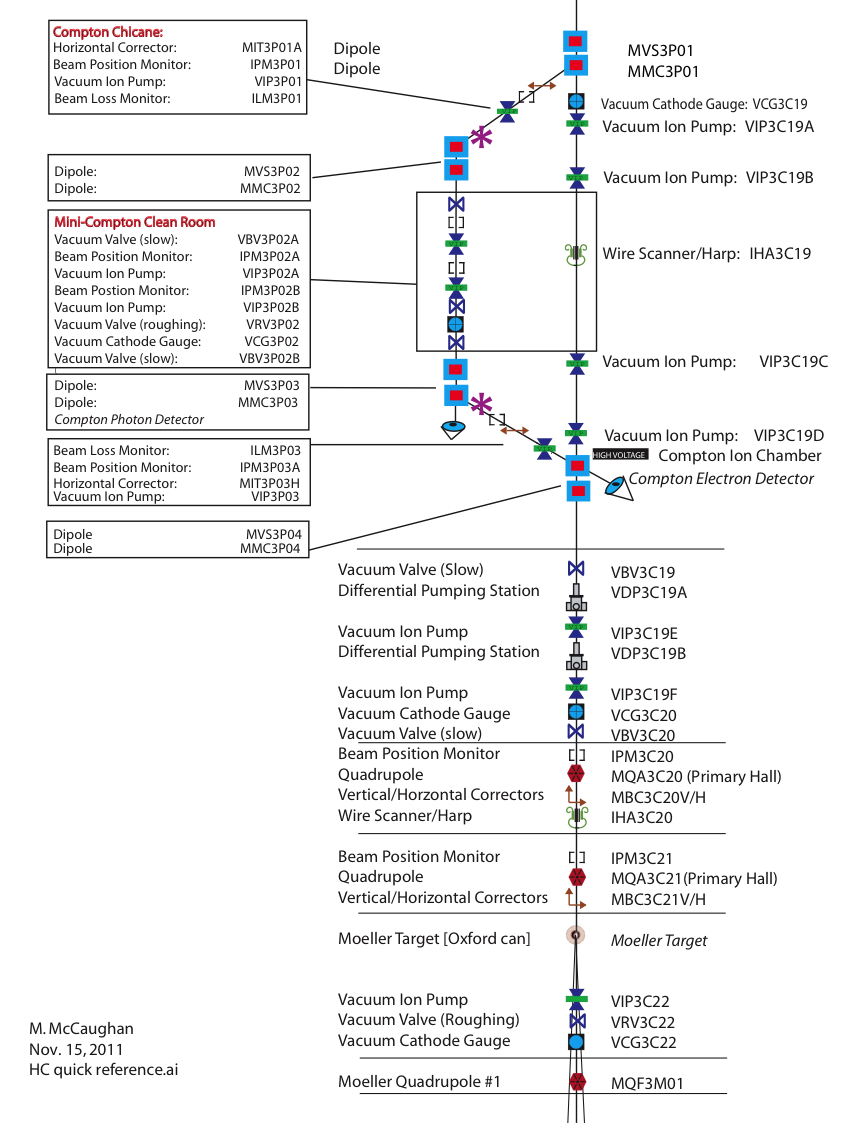
\includegraphics[width=15.0cm]{figures/BeamlineDrawing5}
	\end{center}
	\caption
%	[BeamlineDrawing5.]	
	{Beamline drawing 5.}
	\label{fig:BeamlineDrawing5}
\end{figure}
\end{singlespace}

\begin{singlespace}
\begin{figure}[!h]
	\begin{center}
	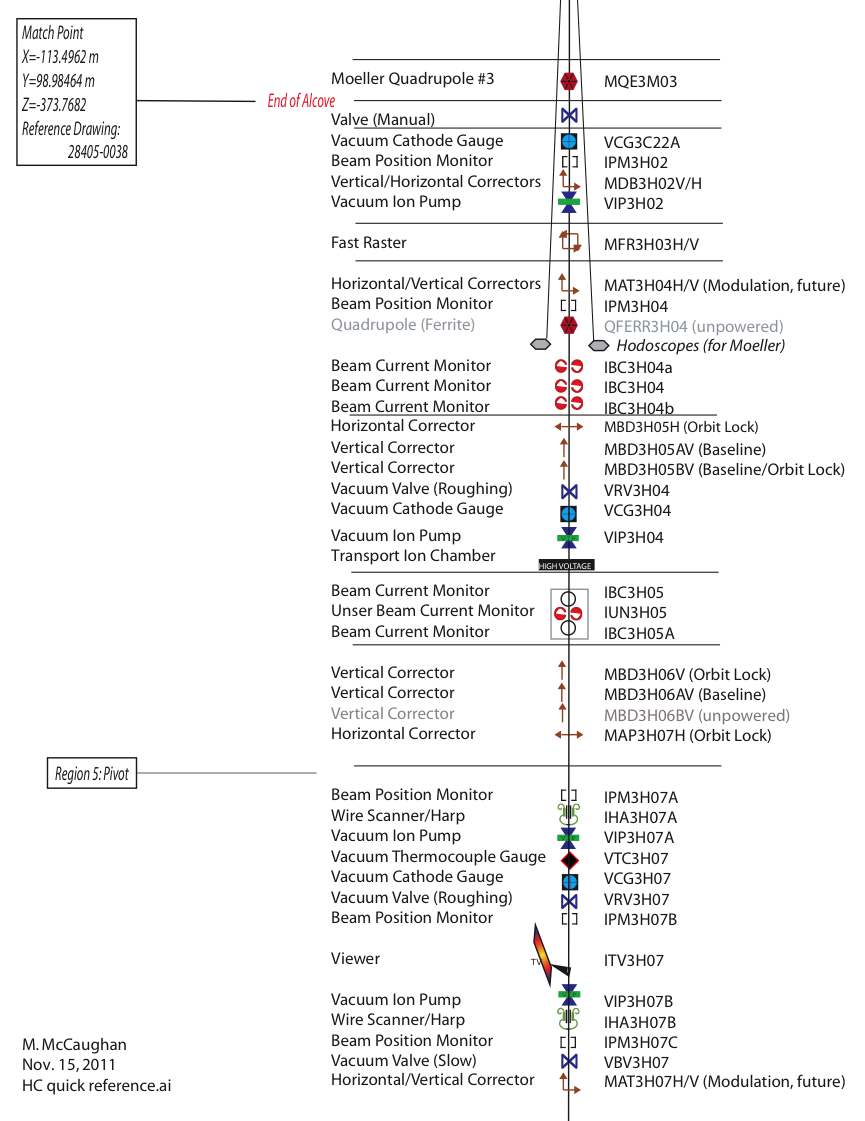
\includegraphics[width=15.0cm]{figures/BeamlineDrawing6}
	\end{center}
	\caption
%	[BeamlineDrawing6.]	
	{Beamline drawing 6.}
	\label{fig:BeamlineDrawing6}
\end{figure}
\end{singlespace}

\begin{singlespace}
\begin{figure}[!h]
	\begin{center}
	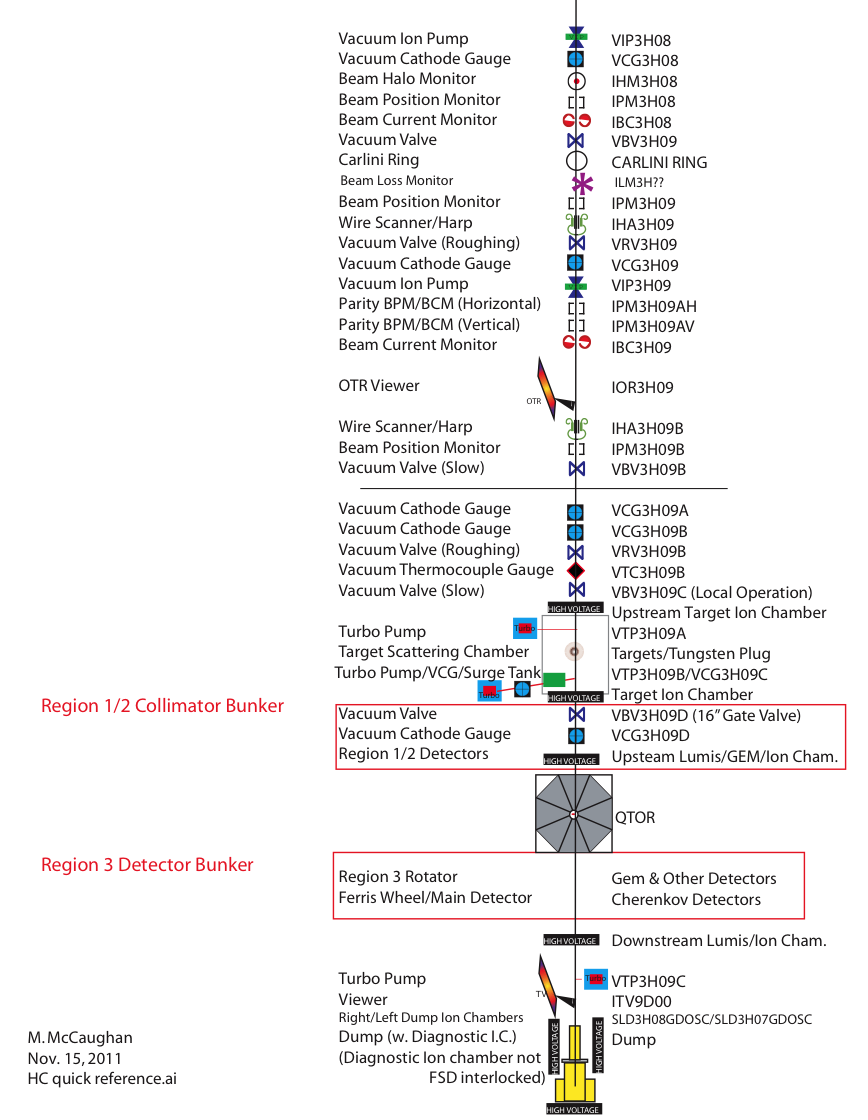
\includegraphics[width=15.0cm]{figures/BeamlineDrawing7}
	\end{center}
	\caption
%	[BeamlineDrawing7.]	
	{Beamline drawing 7.}
	\label{fig:BeamlineDrawing7}
\end{figure}
\end{singlespace}

